\documentclass[11pt,a4paper,oldfontcommands,openany]{memoir}
\usepackage{graphicx}
\usepackage[]{color}
\usepackage{courier}
\usepackage[usenames,dvipsnames]{xcolor}
\usepackage[breakable, theorems, skins]{tcolorbox}
\usepackage[]{media9}
\usepackage{lipsum}
\tcbset{enhanced}
%% maxwidth is the original width if it is less than linewidth
%% otherwise use linewidth (to make sure the graphics do not exceed the margin)
\makeatletter
\def\maxwidth{ %
  \ifdim\Gin@nat@width>\linewidth
    \linewidth
  \else
    \Gin@nat@width
  \fi
}
\makeatother

\DeclareRobustCommand{\mybox}[2][gray!15]{%
\begin{tcolorbox}[   %% Adjust the following parameters at will.
        breakable,
        left=0pt,
        right=0pt,
        top=0pt,
        bottom=0pt,
        colback=#1,
        colframe=#1,
        width=\dimexpr\textwidth\relax, 
        enlarge left by=0mm,
        boxsep=5pt,
        arc=0pt,outer arc=0pt,
        ]
        #2
\end{tcolorbox}
}


\definecolor{fgcolor}{rgb}{0.345, 0.345, 0.345}
\newcommand{\hlnum}[1]{\textcolor[rgb]{0.686,0.059,0.569}{#1}}%
\newcommand{\hlstr}[1]{\textcolor[rgb]{0.192,0.494,0.8}{#1}}%
\newcommand{\hlcom}[1]{\textcolor[rgb]{0.678,0.584,0.686}{\textit{#1}}}%
\newcommand{\hlopt}[1]{\textcolor[rgb]{0,0,0}{#1}}%
\newcommand{\hlstd}[1]{\textcolor[rgb]{0.345,0.345,0.345}{#1}}%
\newcommand{\hlkwa}[1]{\textcolor[rgb]{0.161,0.373,0.58}{\textbf{#1}}}%
\newcommand{\hlkwb}[1]{\textcolor[rgb]{0.69,0.353,0.396}{#1}}%
\newcommand{\hlkwc}[1]{\textcolor[rgb]{0.333,0.667,0.333}{#1}}%
\newcommand{\hlkwd}[1]{\textcolor[rgb]{0.737,0.353,0.396}{\textbf{#1}}}%

\usepackage{framed}
\makeatletter
\newenvironment{kframe}{%
 \def\at@end@of@kframe{}%
 \ifinner\ifhmode%
  \def\at@end@of@kframe{\end{minipage}}%
  \begin{minipage}{\columnwidth}%
 \fi\fi%
 \def\FrameCommand##1{\hskip\@totalleftmargin \hskip-\fboxsep
 \colorbox{shadecolor}{##1}\hskip-\fboxsep
     % There is no \\@totalrightmargin, so:
     \hskip-\linewidth \hskip-\@totalleftmargin \hskip\columnwidth}%
 \MakeFramed {\advance\hsize-\width
   \@totalleftmargin\z@ \linewidth\hsize
   \@setminipage}}%
 {\par\unskip\endMakeFramed%
 \at@end@of@kframe}
\makeatother

\definecolor{shadecolor}{rgb}{.97, .97, .97}
\definecolor{messagecolor}{rgb}{0, 0, 0}
\definecolor{warningcolor}{rgb}{1, 0, 1}
\definecolor{errorcolor}{rgb}{1, 0, 0}
\newenvironment{knitrout}{}{} % an empty environment to be redefined in TeX

\usepackage{alltt}
\setlength{\parindent}{0pt} % Remove indent at new paragraphs
\setcounter{secnumdepth}{4}  % Remove section numbering at certain depth # If zero, then no numbering of sections
\setcounter{tocdepth}{4} % Determines number of subsections that will have tabs
\usepackage{tabu}
\usepackage{url}

\usepackage[round]{natbib}   % omit 'round' option if you prefer square brackets
\bibliographystyle{plainnat}

\usepackage{fixltx2e}
%\usepackage{graphicx}	% For external pictures
\usepackage{float}
\usepackage{subfig}	% Add subfigures within figures
\usepackage{verbatim}
\usepackage[colorlinks=true,linkcolor=blue,citecolor=blue,urlcolor=blue]{hyperref}
\usepackage{amssymb,amsbsy,amsmath}
\usepackage{epsfig}
\usepackage[left=3cm,top=3cm,bottom=3.5cm,right=3cm]{geometry} % For easy document margins
%\usepackage{fancyhdr} % For customization of header/footer
\usepackage{adjustbox}
\usepackage{framed}
\usepackage{enumitem}
\usepackage{caption}
\numberwithin{equation}{section} % Equation numbers relative to sections

%%%%% NEW ADDED FROM THESIS.TEX %%%%% 
\usepackage[utf8]{inputenc}
\usepackage[T1]{fontenc}
\usepackage{microtype}
%\usepackage[dvips]{graphicx}
%\usepackage{times} %clash
%%%%%%%%%%%%%%%%%%%%%%%%%%%%%%%%%%%%%%%% 
\newcommand{\code}[1]{{\texttt{#1}}}
\newcommand{\pkg}[1]{{\texttt{#1}}}
\newcommand{\class}[1]{{\textit{#1}}}
\newcommand{\R}{{\normalfont\textsf{R }}{}}
\IfFileExists{upquote.sty}{\usepackage{upquote}}{}


\begin{document}

\sloppy

%%%%%%%%%%%%%%%%%%%%% TITLE PAGE %%%%%%%%%%%%%%%%%%%%%

{
\centering
~\vspace{\fill}

\vspace{2.5cm}

{\LARGE Thesis Proposal}

\vspace{1cm}

{\LARGE\textbf{Visualization methods for genealogical and RNA-sequencing datasets}}

\vspace{1cm}

{\LARGE Lindsay Rutter}

\vspace{4cm}

{\LARGE Program of Study Committee:}

\vspace{1cm}

{\LARGE Dianne Cook (Major Professor)}

\vspace{.25cm}

{\LARGE Amy Toth (Major Professor)}

\vspace{.25cm}

{\LARGE Heike Hofmann}

\vspace{.25cm}

{\LARGE Daniel Nettleton}

\vspace{.25cm}

{\LARGE James Reecy}

\vspace{2.5cm}

{\centerline{\large May 16, 2016}}
}

\clearpage
%\cleardoublepage

%%% CHAPTER'S STYLE
\chapterstyle{bianchi}
\setsecheadstyle{\Large\bfseries\sffamily\raggedright}
\setsubsecheadstyle{\large\bfseries\sffamily\raggedright}
\setsubsubsecheadstyle{\bfseries\sffamily\raggedright}
%%%%%%%%%%%%%%%%%%%%%%%%%%%%%%%%%%%%

\tableofcontents

\setlength{\parskip}{10pt} % Inter-paragraph spacing

%%% ADDED FROM THESIS.TEX %%%%%%%%%
\OnehalfSpacing

\chapter{Introduction}
%%%%%%%%%%%%%%%%%%%%%%%%%%%%%%%%%%%%%%%%%%%%%%%%%%%%%%%%%%%%%%%%%%%
%%%%%%%%%%%%%%%%%%%%%%%%%%%%%%%%%%%%%%%%%%%%%%%%%%%%%%%%%%%%%%%%%%%
\section{Background to data visualization}

The problem with only applying traditional modeling approaches to data is that these models are replete with assumptions that they alone cannot call into question. Fortunately, visualization enables analysts to see things they may not have expected with traditional modeling. By plotting the data, analysts can determine whether or not the applied models are sensible; they can work between visualizations and modeling, enhancing the models based on feedback from the visuals. In sum, graphics are essential for analysts to check the quality of the data, assess the model diagnostics, and compare results from different methods.

%%%%%%%%%%%%%%%%%%%%%%%%%%%%%%%%%%%%%%%%%%%%%%%%%%%%%%%%%%%%%%%%%%%
%%%%%%%%%%%%%%%%%%%%%%%%%%%%%%%%%%%%%%%%%%%%%%%%%%%%%%%%%%%%%%%%%%%
\section{Problems to be addressed}

Genealogical data has a standardized type of display known as a pedigree chart, which we introduce in Section \ref{sec:litReview} (\citealt{ped}). While this visual plot is useful for certain genealogical datasets, it is not useful for many genealogical datasets, particularly agricultural ones that are used for breeding purposes. We address this problem by introducing a new type of plot to display the paths between the ancestors and descendants constrained by generation for an individual of interest, which could otherwise not be accomplished with a pedigree chart. This new plot (and other plots) are introduced in Chapter \ref{sec:ggenealogy}.

There are popular plotting tools for analyzing RNA-sequencing data, but there are less popular tools that could be more helpful for RNA-sequencing analysis. We strive to work on the following five uncommon plotting types that could be useful for better understanding RNA-sequencing data, and we show our work-in-progress toward these goals in Chapters \ref{sec:clustering} and \ref{sec:sigtest}:

\clearpage

\begin{enumerate}
\item \textbf{Parallel coordinate plots}:

In gene expression data analysis, we are striving to find relative patterns. Side-by-side boxplots are often used for this purpose, but they can hide potential problems that could still be lurking in the data after normalization. This is because most RNA-sequencing normalization methods are conducted at the sample-level, and side-by-side boxplots do not show connections between the samples. Consequently, boxplots may deceive analysts to believe that the normalization succeeded in cases where alternative plots (such as parallel coordinate plots) would have otherwise indicated that the normalization was in fact unsuccessful due to the presence of inconsistencies (crossings) between replicates. For this reason, parallel coordinate plots (\citealt{origPCP}, \citealt{origPCP2}) are an essential visual tool when checking the initial normalization process of RNA-sequencing analysis. If the normalization is adequate, then the connections between replications should be flat, and we should only see crossings between treatment groups.

The tools currently available for constructing parallel coordinate plots to assess RNA-sequencing data are severely limited: Namely, the large number of genes present can cause constraints in space and time. With one line being drawn for each gene, our resulting plots will have too many lines being drawn to even view patterns of interest in the first place. Moreover, the construction of these plots can be consuming in computation and time, often requiring analysts to wait for minutes before they can view the output. Even though popular tools to visualize parallel coordinate plots (such as the \code{ggparcoord} function in the \code{GGally} package) can be very useful for many datasets, they are not always helpful for large RNA-sequencing datasets (\citealt{ggally}). As a result, our goal is to develop a new approach that both quickly and meaningfully displays the key pieces of information for RNA-sequencing data with parallel coordinate plots. 

\item \textbf{Pairwise scatterplots}:

We aim to develop visuals that can effectively plot replicates against each other. We can do this by generating pairwise scatterplots for replicates, using the \code{scatmat()} function of the \code{GGally} package (\citealt{ggally}). If the data is high quality, then we would expect negligent differences between read counts across replicates. This would result in a scatterplot where the read counts from the two replicates fall along the x=y relationship. Deviations from this expectation would indicate a quality problem with the data.

With this second goal we face the same challenges that we did with the first goal: We have a plotting algorithm that is not tailored to deal with the vastly sized datasets like RNA-sequencing data. As a result, we again face space (overplotting) and time (computational speed) constraints, and our goal would be to tailor the scatterplot matrix to adapt to large amounts of data. In addition, we must now recognize that the few data points along the perimeter of the x=y relationship that we can see may be misleading. Hence, we would want to develop guidelines in terms of what denotes a high-quality dataset where read counts are similar between replicates and different between treatments. 

\item \textbf{Replicate line plots}:

We aim to build upon a new type of plot for gene expression analysis called the replicate line plot, which was developed fairly recently (\citealt{jds}). This plot can be used to visually mine for genes that have small variability in replicates but large variability across treatments. While this plot has been developed and shown to be useful for two replicates, we would wish to expand upon this so that it can be used for more than two replicates. We show an example from the original study that introduced replicate line plots in Figure \ref{fig:porcupine} (\citealt{jds}).

\begin{figure}[H]
\centering
    \begin{framed}
    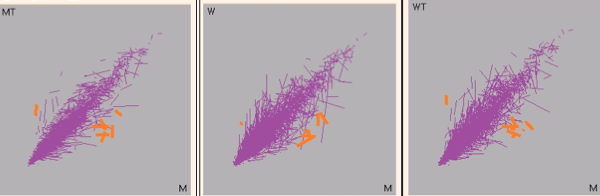
\includegraphics[width=0.8\textwidth]{porcupine}
    \end{framed}
    \caption{Three replicate line plots in which genes of interest (show low variability across replicates but high variability across treatments) are highlighted in orange. For example, in the plot on the left, there are two treatments (MT and M) that each have two replicates. If a gene shows high variability between the two treatments, then it would fall away from the x=y line. If a gene shows low variability between replicates, then the distance between the two replicates will be short. Hence, the genes of interest will be visually represented as the orange ones that are short in length and deviate from the x=y line.}
    \label{fig:porcupine}
\end{figure}

\item \textbf{Single gene plots}:

We plan to develop plots that allow users to look in more detail at individual genes of interest. For instance, while a user may generate a subset of genes from a clustering analysis, they may wish to view the read count across the samples for each of these genes in a visual manner. This may allow a user to quickly sift through the subset of genes and visually determine which ones may truly be of interest.

\item \textbf{Permutation testing plots}:

We aim to develop permutation testing plots for differentially expressed genes. Even if a subset of genes may be deemed statistically significantly differentially expressed, we may wish to see what this might look like if we permuted. We could obtain confidence bands and see if the top differentially expressed genes are signal or noise.

\end{enumerate}

%%%%%%%%%%%%%%%%%%%%%%%%%%%%%%%%%%%%%%%%%%%%%%%%%%%%%%%%%%%%%%%%%%%
%%%%%%%%%%%%%%%%%%%%%%%%%%%%%%%%%%%%%%%%%%%%%%%%%%%%%%%%%%%%%%%%%%%

\section{Literature review}
\label{sec:litReview}
%%%%%%%%%%%%%%%%%%%%%%%%%%%%%%%%%%%%%%%%%%%%%%%%%%%%%%%%%%%%%%%%%%%
\subsection{Visualization methods for genealogical data}

Publishing in the open source \pkg{R} statistical programming language allows for tools to be distributed and modified at ease, encourages cross-platform collaboration, and provides a foundation for effective and aesthetic data visualization from the grammar of graphics. There are several useful \pkg{R} packages that offer tools for analyzing and visualizing genealogical datasets. Here, we introduce these packages, and emphasize the shortcomings for which our package \pkg{ggenealogy} brings to this collection of work.

The \pkg{R} package \pkg{pedigree} is named after the standardized chart used to study human family lines, and sometimes used to select breeding of animals, such as show dogs (\citealt{ped}). This package does provide tools that perform methods on parent-child datasets, such as rapidly determining the generation count for each member in the pedigree. However, it does not provide any visualization tools.

Another \pkg{R} package called \pkg{kinship2} does produce basic pedigree charts (\citealt{kin}). In Figure \ref{fig:kinshipFig}, we provide an example pedigree chart from the \pkg{kinship2} package vignette. This pedigree chart adheres to the standard set of symbols used for visualizing genealogical structures: Males are represented with squares and females with circles. Parents are connected to each other by horizontal lines, and to their children by vertical lines. Siblings are connected by horizontal sibship lines. Even though this standard pedigree chart creates powerful charts that can be applied across many applications, it cannot provide unequivocal information in situations where inter-generational breeding occurs, as is often the case in agronomic genealogical lineages.

We demonstrate how the standardized pedigree charts in the \pkg{kinship2} package generate ambiguous results in such scenarios by superimposing a hypothetical inter-generational breeding case in Figure \ref{fig:kinshipFig}. In that figure, each generation is defined by its position on the vertical axis, with the first generation containing individuals 201 and 202. We superimposed green-highlighted individual 215 onto the pedigree chart for explanatory purposes. Its parents are individuals 201 and 206, which are from generations one and two, respectively, and have a parent-child relationship between themselves. As an offspring of a parent-child relationship, individual 215 is both a second and third generation individual. Hence, individual 215 should be displayed in both second and third generational positions on the vertical axis. However, standard pedigree tools only allow for an individual to be displayed once. As a result, in special cases where inter-generational breading occurs, such as in agronomic applications, standardized tools for visualizing genealogical information ambiguously portray the genealogical dataset.

\begin{figure}[H]
    \begin{framed}
    \centering
    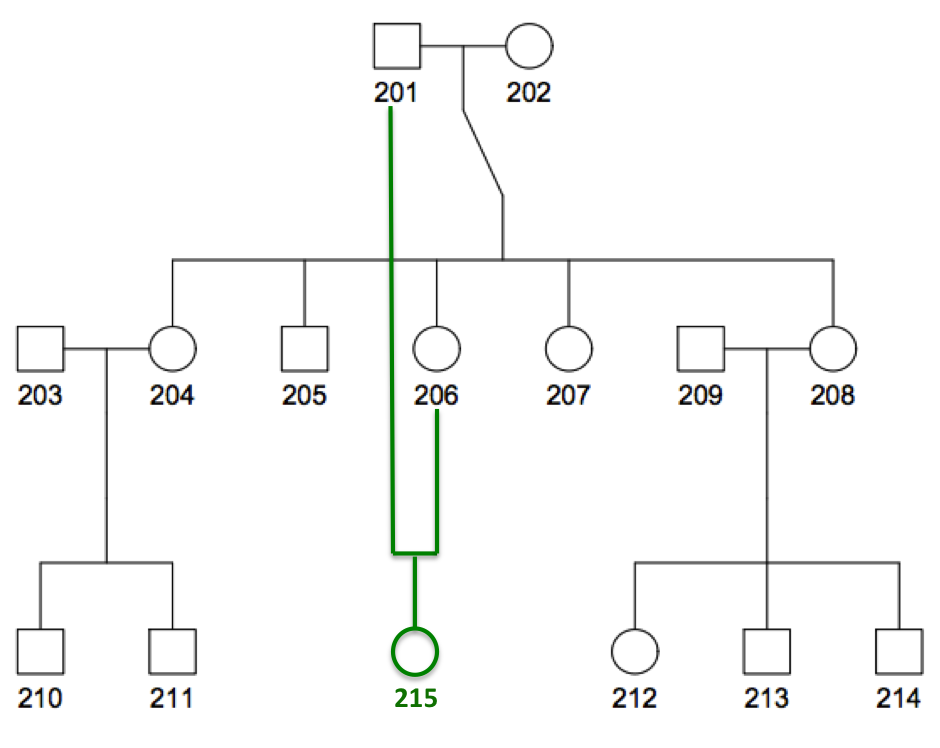
\includegraphics[width=0.65\textwidth]{kinshipFig}
    \end{framed}
    \caption{Example pedigree chart from the \pkg{kinship2} package, where the vertical axis denotes generation count. We superimposed green-highlighted individual 215 for explanatory purposes. As an offspring of a parent-child relationship, individual 215 is both a second and third generation individual. Hence, it should be displayed twice on the vertical axis, once for each of its generation counts. However, standard pedigree tools only allow for an individual to be displayed once, leading to ambiguous portrayal of the genealogical dataset.}
    \label{fig:kinshipFig}
\end{figure}

In addition, popular graph drawing software such as \pkg{GraphViz} and \pkg{Cytoscape} can be used to visualize genealogical structures (\citealt{graphvizCit}, \citealt{cytoscapeCit}). Graphs are defined as objects with sets of nodes and edges, where sets indicate that their comprised elements cannot be repeated. In other words, graphical structures do not allow for repeated nodes, and hence, as is the case with the aforementioned \pkg{R} packages, these popular graph plotting software cannot precisely portray the genealogical dataset in cases of inter-generational breeding.

We again illustrate this problem in Figure \ref{fig:Graph} with an example genealogy using popular graph drawing software like \pkg{GraphViz} and \pkg{Cytoscape}. Here, generation count is denoted by the vertical axis. As was shown in Figure \ref{fig:kinshipFig}, here too we superimpose a green node that has parents from two different generations. This green node is both a second and third generation individual, and should be displayed in both corresponding generation positions on the vertical axis. However, standard graph visualization tools only allow for a given node to be displayed once. As a result, this green node must be ambiguously positioned in either the second or third generation position; in the figure, it is denoted as a third generation individual. In Chapter 3, we will demonstrate \pkg{ggenealogy} plots that can remedy these problems.

\begin{figure}[H]
    \begin{framed}
    \centering
    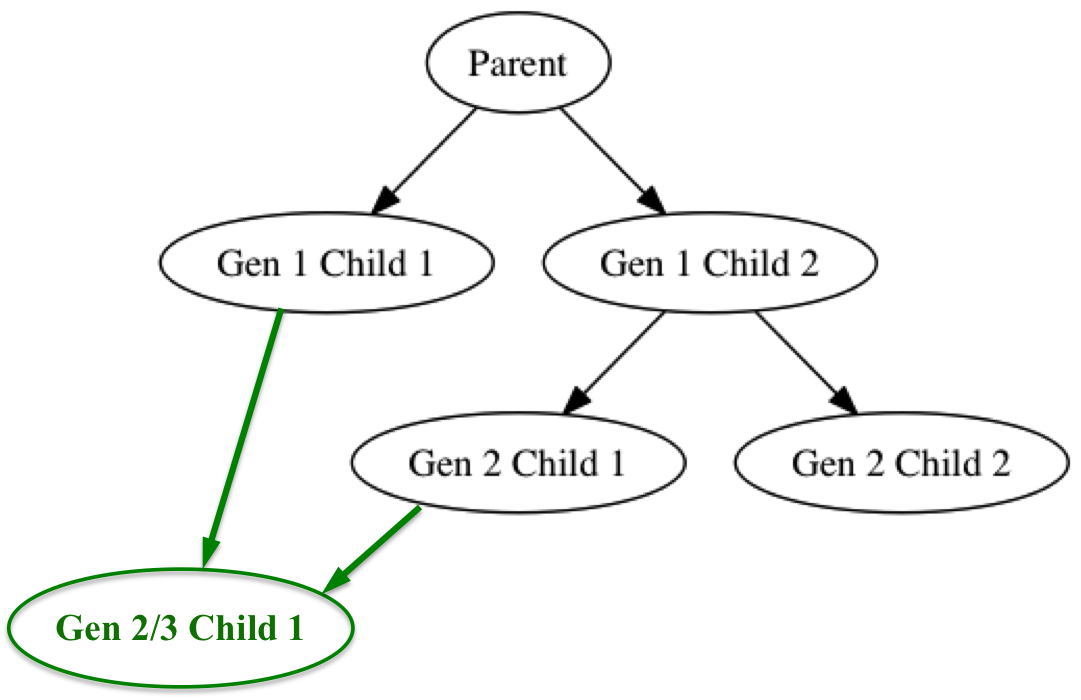
\includegraphics[width=0.6\textwidth]{Graph}
    \end{framed}
    \caption{Example genealogical display using popular graph software like \pkg{GraphViz} and \pkg{Cytoscape}, with generation count denoted by the vertical axis. As was shown in Figure \ref{fig:kinshipFig}, the green node has parents from two different generations, and hence must be ambiguously positioned as one of two generation counts.}
    \label{fig:Graph}
\end{figure}

%%%%%%%%%%%%%%%%%%%%%%%%%%%%%%%%%%%%%%%%%%%%%%%%%%%%%%%%%%%%%%%%%%%
\subsection{Visualization methods for RNA-sequencing data}

Previous studies have provided sound evidence that gene expression data is most effectively explored by using graphical and numerical approaches in a complementary fashion (\citealt{extra2}, \citealt{extra1}, \citealt{extra4}). The authors of one study demonstrated this finding by applying modeling and visualization tools to simulated and real microarray data (\citealt{jds}). Through the use of plots, they determined that their initial models were inappropriate and needed improvement, and that the data quality was questionable and needed relabeling.

Moreover, they demonstrated that some of the most common plots for gene expression data are rife with problems, while some of the less popular plots are useful. In one example, they showed that heat maps are commonly-used, but they do not allow users to detect outlying genes. In contrast, scatterplots can allow for outlier detection. Furthermore, they introduced a new type of plot called the replicate line plot, which can be used to visually mine for genes that show low variability in read counts between replicates but high variability in read counts between treatments. The authors also showed the importance of interaction on plots for gene expression analysis; they used GGobi (\citealt{ggobi}, \citealt{ggobi2}, \citealt{ggobi3}) to generate direct manipulation and linking between various multivariate plots to display the data. Interactive plots for multivariate data could also be accomplished with the use of projections (\citealt{extra3}).

%%%%%%%%%%%%%%%%%%%%%%%%%%%%%%%%%%%%%%%%%%%%%%%%%%%%%%%%%%%%%%%%%%%
%%%%%%%%%%%%%%%%%%%%%%%%%%%%%%%%%%%%%%%%%%%%%%%%%%%%%%%%%%%%%%%%%%%
\section{Overview of thesis research}

%%%%%%%%%%%%%%%%%%%%%%%%%%%%%%%%%%%%%%%%%%%%%%%%%%%%%%%%%%%%%%%%%%%

In Chapter \ref{sec:ggenealogy}, we introduce \textbf{\pkg{ggenealogy}} (\citealt{ggen}), a developing \pkg{R} software package that provides tools for searching through genealogical data, generating basic statistics on their graphical structures using parent and child connections, and displaying the results. The package allows users to draw the genealogy in relation to variables related to the nodes, and to determine and display the shortest path distances between the nodes. Production of pairwise distance matrices and genealogical diagrams constrained on generation are also available in the visualization toolkit. We have tested the tools on a dataset with milestone cultivars of soybean varieties (\citealt{soybean}) as well as on a web-based database of the academic genealogy of mathematicians (\citealt{mgp}).

Susan VanderPlas began the original work for this package and developed most features in the \code{plotAncDes()} function. The software package has been available on the Comprehensive \pkg{R} Archive Network since March 2015 (\citealt{ggen}). In August 2015, a paper introducing the \pkg{ggenealogy} software package received a student paper competition award from the Statistical Computing and Graphics Section of the American Statistical Association. Currently, we are preparing to submit another paper describing the software package to the Journal of Statistical Software. We also aim to release a second version of the package as we have added interactive plotting tools that were not available in the first version.

In Chapter \ref{sec:clustering}, we show what we have accomplished toward developing visualization methods for clustering analysis of RNA-sequencing data. We use a soybean example dataset with treatments of iron-poor and iron-rich conditions. On the clustered data, we use both scatterplot matrices and parallel coordinate plots to determine which clusters are of interest. We also use individual gene plots to determine if there subsets of genes within clusters of interest that should be reconsidered.

In Chapter \ref{sec:sigtest}, we demonstrate some of our work-in-progress toward developing visualization methods for significance testing of RNA-sequencing data. We use a paper wasp example dataset with treatments of antennal drumming and nutrition. We use individual transcript plots to determine if the top statistically-significantly differentially expressed transcripts appear to show differences in read counts across the treatments.

In Chapter \ref{sec:timeline}, we tabulate the completed work, the scheduled deliverables for thesis completion, and other work performed outside of thesis work.



%%%%%%%%%%%%%%%%%%%%%%%%%%%%%%%%%%%%%% CHAPTER %%%%%%%%%%%%%%%%%%%%%%%%%%%%%%%%%%%%%% 
%%%%%%%%%%%%%%%%%%%%%%%%%%%%%%%%%%%%%%%%%%%%%%%%%%%%%%%%%%%%%%%%%%%%%%%%%%%%%%%%%%%%%  
 
\chapter{Visualization methods for genealogical datasets}
\label{sec:ggenealogy}

\section{Introduction}

Genealogy is the study of parent-child relationships. By tracing through parent-child lineages, genealogists can study the histories of features that have been modified over time. Comparative geneticists, computational biologists, and bioinformaticians commonly use genealogical tools to better understand the histories of novel traits arising across biological lineages. For example, desirable modifications in crops could include an increase in protein yield or an increase in disease resistance, and genealogical structures could be used to assess how these desirable traits developed. At the same time, genealogical lineages can also be used to assess detrimental features, such as to determine the origin of hazardous traits in rapidly-evolving viruses.

Genealogical structures can also serve as informative tools outside of a strict biological sense. For instance, we can trace mentoring relationships between students and dissertation supervisors with the use of academic genealogies. This can allow us to understand the position of one member in the larger historical picture of academia, and to accurately preserve past relationships for the knowledge of future generations. Similarly, linguistic genealogies can be used to decipher the historical changes of vocabulary and grammatical features across related languages. In short, there is a diverse array of disciplines that can elicit useful information about features of interest by using genealogical data.

In all these examples, the genealogical relationships can be represented visually. Access to various types of plotting tools can allow scientists and others to more efficiently and accurately explore features of interest across the genealogy. We introduce here a developing visualization toolkit that is intended to assist users in their exploration and analysis of genealogical structures. In this paper, we demonstrate the main tools of the software package \pkg{ggenealogy} using two example genealogical datasets, one of soybean cultivars (\citealt{soybean}) and the other of academic mathematicians (\citealt{mgp}).

\section{Example datasets}
\label{exData}

The \pkg{ggenealogy} package comes with two example datasets, one comprises a soybean genealogy and the other comprises an academic statistician genealogy. We will introduce both example datasets to demonstrate some of the tools available in the software.

\subsection{Soybean genealogy}

We start with the soybean genealogy, which is available as a data frame structure with 390 rows and five columns. These data were collected from field trials, genetic studies, and United States Department of Agriculture (USDA) bulletins, and date as early as the first decade of the 1900s. They contain information on the copy number variants, single nucleotide polymorphisms, and protein content for each of the varieties, although we removed that information for a succinct example dataset. In this context, the software could ideally be used by agronomists who wish to study how soybean varieties are related. By referencing the visualization of the genealogical structure, these scientists may better understand genetic testing results - in this particular dataset, in terms of copy number variants, single nucleotide polymorphisms, protein content, and yield - and use that knowledge in future breeding decisions.

Each row contains information about a particular child soybean variety, including the name of the child, its yield, the year it was released, whether or not its release year was imputed, and the name of its parent. It should be noted that it typically requires many crosses over the span of one to two decades to develop a new variety that has introduced a desired trait and/or removed an undesired trait. Hence, the release year variable in this dataset represents the year in which the variety was released to the public after its development period. While the name of the child is required, the other four columns can have missing values (which are represented in \pkg{R} with the symbol NA for "not available"). As a result, while each row does contain information about a particular child soybean variety, whether or not a given row also contains information about a parent-child relationship between a pair of soybeans depends on whether or not the parent column has a missing value.

In total, there are 230 soybean varieties in the dataset, 206 of which are children and 165 of which are parents. There are soybeans that are both children and parents. Of the children, 156 have two parents, 28 have one parent, and 22 have zero parents. There are 340 parent-child relationships in the dataset.

We can load the example dataset of soybean genealogy (\code{sbGeneal}) and examine its structure. 

\mybox{
\texttt{R> install.packages("ggenealogy")}\\
\texttt{R> library("ggenealogy")}\\
\texttt{R> data(sbGeneal)}\\
\texttt{R> str(sbGeneal)}
}

\mybox[green!10]{
\texttt{'data.frame':	390 obs. of  5 variables:}\\
\texttt{\$ child       : chr  "5601T" "Adams" "A.K." "A.K. (Harrow)" ...}\\
\texttt{\$ year        : num  1981 1948 1910 1912 1968 ...}\\
\texttt{\$ yield       : int  NA 2734 NA 2665 NA 2981 2887 2817 NA NA ...}\\
\texttt{\$ year.imputed: logi  TRUE FALSE TRUE FALSE FALSE FALSE ...}\\
\texttt{\$ parent      : chr  "Hutcheson" "Dunfield" NA "A.K." ...}
}

\subsection{Academic genealogy of statisticians}

The \pkg{ggenealogy} package also comes with an academic genealogy of statisticians; this dataset is in the form of a data frame with 8165 rows and six columns. To develop this later dataset, we contacted the Math Genealogy Project (\citealt{mgp}), a web-based database for the genealogy of academic mathematicians. This database, which currently contains almost 200,000 entries, is a service of the North Dakota State University Department of Mathematics and the American Mathematical Society. The Mathematics Genealogy Project contact provided us a Structured Query Language (SQL) export, and we used PostgreSQL to query the database (\citealt{psql}).

Each entry in the database contained 26 variables pertaining to an individual who received a graduate-level academic degree in mathematics. One of these variables was called "msc" (Mathematics Subject Classification), and we selected only those entries that contained a value of 62 for this variable (coded as "Statistics"). Furthermore, we only retained entries that had a parent if that parent was also in the field of "Statistics". Hence, in our parent-child relationships, both the child and the parent received postbaccalaureate degrees in statistics, and the parent was the academic advisor to the child. This process resulted in 8995 entries, which we reduced to 8165 entries by removing duplicate entries. With the final data frame of 8165 entries, we only maintained six of the original 26 variables. 

Each row of the final data frame contains information about a particular child who received a graduate-level academic degree in statistics, including the name of the child, the year the child obtained the degree, the country and school from which the child obtained the degree, the thesis title of the degree awarded to the child, and the name of its parent. There are no missing values for the country and school from which the child received its degree or the name of the child; however, some of the years contain missing values (NA), and some of the parent and thesis names contain empty strings (""). As a result, while each row does contain information about a particular child, whether or not a row also contains information about a parent-child relationship between a pair of academic statisticians depends on whether or not the parent column has an empty string.
 
In total, there are 7122 individuals in the dataset, 7122 of which are children and 872 of which are parents. Every parent is also a child, but not every child is also a parent. Of the children, two have four parents, ten have three parents, 226 have two parents, 2801 have one parent, and 4083 have no parents. There are 3291 parent-child relationships in the dataset.

We can load the example dataset of academic genealogy of statisticians (\code{statGeneal}) and examine its structure. 

\mybox{
\texttt{R> data(statGeneal)}\\
\texttt{R> dim(statGeneal)}
}

\mybox[green!10]{
\texttt{[1] 8165    6}
}

\mybox{
\texttt{R> colnames(statGeneal)}
}

\mybox[green!10]{
\texttt{[1] "child"   "parent"  "year"    "country" "school"  "thesis"}
}

\section{Genealogical input format}

As is the case with both example data files introduced above, \pkg{ggenealogy} requires that the genealogy input file is a data frame structure with at least two columns. One column must be labeled "child", and each case in that column must be of type character. The other column must be labeled "parent," and each case in that column must either be of type character, type NA, or type "". At this point, any \pkg{ggenealogy} plot that only requires information about parent-child relationships can be used.

However, some \pkg{ggenealogy} plots also make use of quantitative variable values associated with individuals in the genealogy. For these plots, the input data frame should also contain a third column. In both example data files, this column is labeled "year," and each case in that column can either be of type numeric, type NA, or type "". At this point, any \pkg{ggenealogy} plot can be used.

\section{Generating a graphical object}

Most functions in the \pkg{ggenealogy} software package require an input parameter of a graph structure. Therefore, as a preprocessing step, we must first convert our original data frame structure into a graph structure. Below, we read in the \pkg{R} data file \code{sbGeneal} that is included in the package as a sample data set of soybean genealogy.

We now convert it into an \pkg{igraph} object (\citealt{igraph}) \code{sbIG} using the function \code{dfToIG()}.

\mybox{
\texttt{R> sbIG <- dfToIG(sbGeneal)}\\
\texttt{R> sbIG}
}

\mybox[green!10]{
\texttt{IGRAPH UNW- 230 340 -- }\\
\texttt{+ attr: name (v/c), weight (e/n)}\\
\texttt{+ edges (vertex names):}\\
\texttt{ [1] 5601T    --Hutcheson        Adams    --Dunfield} \\       
\texttt{ [3] A.K.     --A.K. (Harrow)    Altona   --Flambeau} \\       
\texttt{ [5] Amcor    --Amsoy 71         Adams    --Amsoy } \\         
\texttt{ [7] Amsoy 71 --C1253            Anderson --Lincoln   } \\     
\texttt{ [9] Bay      --York             Bedford  --Forrest  }\\       
\texttt{[11] Beeson   --Kent             Blackhawk--Richland } \\      
\texttt{[13] Bonus    --C1266R           Bradley  --J74-39  } \\       
\texttt{[15] Bragg    --Jackson          Bragg    --Bragg x D60-7965}\\
\texttt{+ ... omitted several edges}
}

There are many statistics about the \code{sbGeneal} dataset that we may wish to know that cannot easily be obtained through images and tables. The package function \code{getBasicStatistics()} can be called, using the \code{sbIG} object as input. This will return a list of common graph theoretical measurements regarding the genealogical structure. For instance, is the whole structure connected? If not, how many separated components does it contain? In addition to these statistics, the \code{getBasicStatistics()} function will also return the number of nodes, the number of edges, the average path length, the graph diameter, and other graph theoretical information.

\mybox{
\texttt{R> getBasicStatistics(sbIG)}
}

\mybox[green!10]{
\texttt{\$isConnected}\\
\texttt{[1] FALSE}\\

\texttt{\$numComponents}\\
\texttt{[1] 11}\\

\texttt{\$avePathLength}\\
\texttt{[1] 5.333746}\\

\texttt{\$graphDiameter}\\
\texttt{[1] 13}\\

\texttt{\$numNodes}\\
\texttt{[1] 230}\\

\texttt{\$numEdges}\\
\texttt{[1] 340}\\

\texttt{\$logN}\\
\texttt{[1] 5.438079}
}

\section{Plotting a shortest path}

With soybean lineages, it may be useful for soybean breeders to track how two varieties are related to each other via parent-child relationships. Then, any dramatic changes in yield and other measures of interest between the two varieties can be traced across their genetic timeline. The \pkg{ggenealogy} package allows users to select two varieties of interest, and determine the shortest pathway of parent-child relationships between them, using the \code{getPath()} function. This will return a list that contains the variety names and their years in the path.

\mybox{
\texttt{R> pathTN <- getPath("Tokyo", "Narow", sbIG, sbGeneal)}\\
\texttt{R> pathTN}
}

\mybox[green!10]{
\texttt{\$pathVertices}\\
\texttt{[1] "Tokyo"    "Volstate" "Jackson"  "R66-873"  "Narow"}\\   

\texttt{\$yearVertices}\\
\texttt{[1] "1907"   "1942"   "1954.5" "1971.5" "1985"}
}

The returned path object can then be plotted using the \code{plotPath()} function.

\mybox{
\texttt{R> plotPath(pathTN)}
}

\begin{figure}[h]
    \begin{framed}
    \centering
    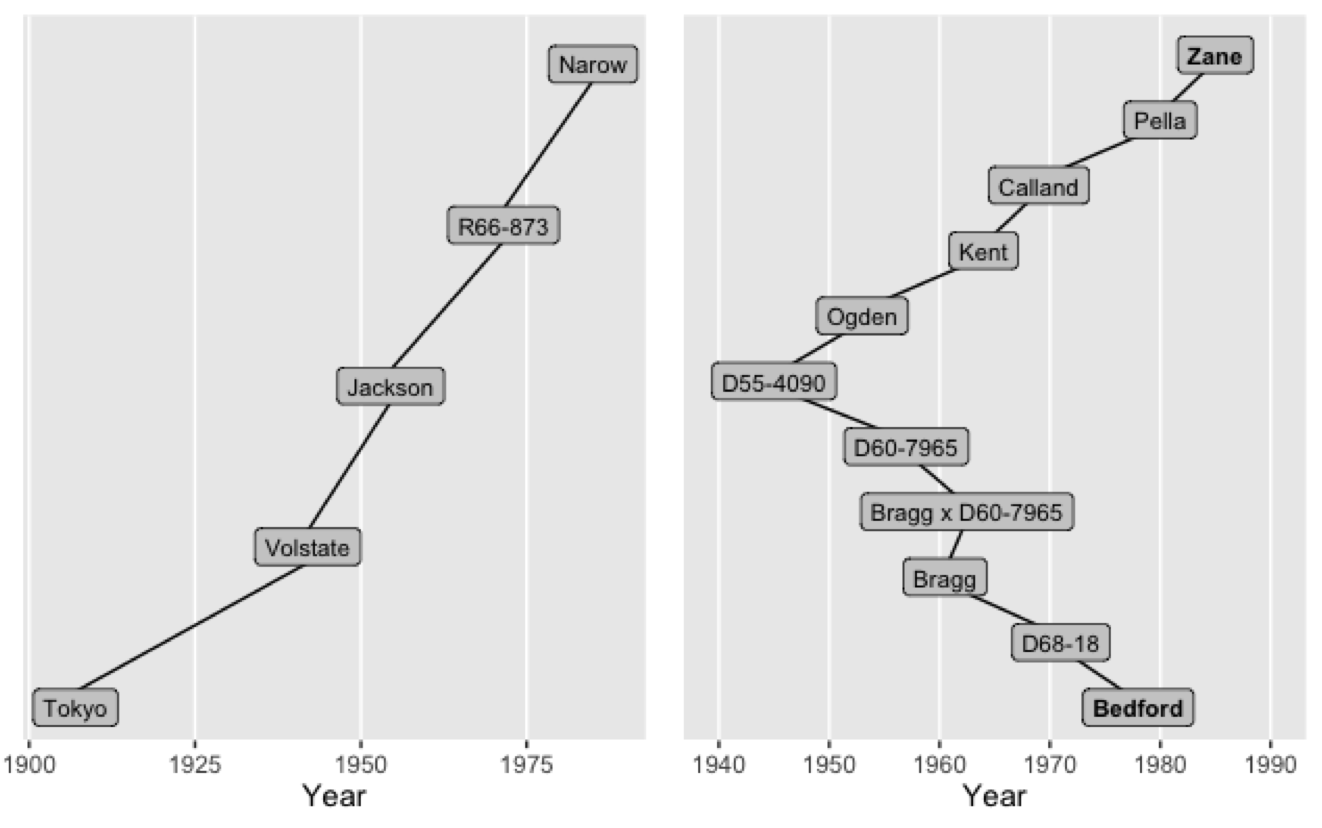
\includegraphics[width=\textwidth]{pathTNZB}
    \end{framed}
    \caption{Left: The shortest path between varieties Tokyo and Narow is strictly composed of a unidirectional sequence of parent-child relationships. Right: The shortest path between varieties Zane and Bedford is not strictly composed of unidirectional parent-child relationships; they instead have a cousin-like relationship.}
    \label{fig:pathTNZB}
\end{figure}

This produces a visual that informs users of all the varieties involved in the shortest path between the two varieties of interest (see left half of Figure \ref{fig:pathTNZB}). In this plot, the release year of all varieties involved in the path are indicated on the horizontal axis, while the vertical axis has no meaning other than to simply to display the labels evenly spaced vertically. The shortest path between varieties \code{Tokyo} and \code{Narow} is composed of a unidirectional series of parent-child relationships, with \code{Tokyo} as the starting ancestor in the early 1900s, \code{Narow} as the most recent descendent in the mid 1980s, and three varieties in between.

Next, we can run the same set of functions on a different pair of varieties. First, a call to the \pkg{ggenealogy} function \code{getYear()} indicates that variety \code{Bedford} was released in 1978 and variety \code{Zane} in 1985.

\mybox{
\texttt{R> getYear("Bedford", sbGeneal)}
}

\mybox[green!10]{
\texttt{[1] 1978}
}

\mybox{
\texttt{R> getYear("Zane", sbGeneal)}
}

\mybox[green!10]{
\texttt{[1] 1985}
}

We can then create a plot showing the shortest path between these two varieties of interest. As this is a longer path, we may also consider setting the \code{fontFace} variable of the \code{plotPath()} to a value of 2, indicating we wish to boldface the two varieties of interest.

\mybox{
\texttt{R> pathBZ <- getPath("Bedford", "Zane", sbIG, sbGeneal)}\\
\texttt{R> plotPath(pathBZ, fontFace = 2)}
}

The resulting plot (right half of Figure \ref{fig:pathTNZB}) allows us to quickly determine that \code{Bedford} is not a parent, grandparent, or any great grandparent of \code{Zane}. Instead, we see that these two varieties are not related through a unidirectional parent-child lineage, but instead have a cousin-like relationship. The oldest common ancestor between \code{Zane} and \code{Bedford} is the variety \code{D55-4090}, which was released in the mid 1940s.

Furthermore, as determined by the figure, for both \code{Zane} and \code{Bedford}, there are four varieties of unidirectional parent-child relationships between each of them and their common ancestor \code{D55-4090}. Hence, any feature of interest that differentiates \code{Zane} and \code{Bedford} (protein content, yield, disease resistance, etc.) can also be examined across these two separate lineage histories.

\section{Superimposing shortest path on tree}

Now that we can create path objects, we may wish to know how those paths are positioned compared to the entire genealogical lineage. For instance, of the documented soybean cultivar lineage varieties, where does the shortest path between two varieties of interest exist? Are these two varieties older compared to the overall data structure? Are they newer? Or, do they span the entire structure, and represent two extreme ends of documented time points?

There is a function available in the \pkg{ggenealogy} package \code{plotPathOnAll()} that can allow users to quickly visualize their path of interest superimposed over all varieties and edges present in the whole data structure. Here we will produce a plot of the shortest path between varieties \code{Tokyo} and \code{Narow} across the entire dataset, as is displayed in Figure \ref{fig:plotTNBin3}.

\mybox{
\texttt{R> plotPathOnAll(pathTN, sbGeneal, sbIG, binVector = 1:3, pathEdgeCol = "red", nodeSize = 2.5, pathNodeSize = 4) + ggplot2::theme(axis.text = ggplot2::element\_text(size = 12), axis.title = ggplot2::element\_text(size = 12))}
}

\begin{figure}%[h]
    \begin{framed}
    \centering
    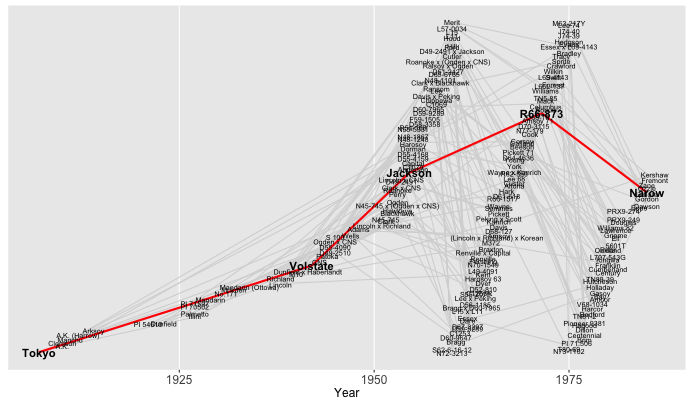
\includegraphics[width=\textwidth]{plotTNBin3}
    \end{framed}
    \caption{The shortest path between Tokyo and Narow, superimposed over the data structure, using a bin size of 3.}
    \label{fig:plotTNBin3}
\end{figure}

In the code above, syntax from the \pkg{ggplot2} package was appended to the \code{plotPathOnAll()} function; this can be done for most \pkg{ggenealogy} functions (\citealt{ggplot2}). While the first three explicit parameters have been introduced earlier in this paper, the fourth parameter (\code{binVector}) requires some explanation. The motivation of the \code{plotPathOnAll()} function is to write node labels on a plot, with the center of each node label constricted on the horizontal axis to its quantitative variable of interest (in this case, year of release). As is the case for the plots before, the vertical axis has no meaning other than providing a plotting area in which to draw the node labels. Unfortunately, for large datasets, this motivation can be a difficult task because the text labels of the varieties can overlap if they are assigned a similar y coordinate, have a similar year (x coordinate), and have long text labels (width of x coordinate).

For each variety, the x coordinate (year) and width of the x coordinate (text label width) cannot be altered, as they provide useful information. However, for each variety, the y coordinate is arbitrary. Hence, in an attempt to mitigate text overlapping, the \code{plotPathOnAll()} function does not randomly assign the y coordinate. Instead, it allows users to partially control the y coordinates with a user-determined number of bins (\code{binVector}).

If the user decides to produce a plot using three bins, as in the example code above, then the varieties are all grouped into three bins based on their year values. In other words, there will be bin 1 (the "oldest bin") which includes the one-third of varieties with the oldest years of release, bin 2 (the "middle bin"), and bin 3 (the "youngest bin"). Then, in order to decrease text overlap, the consecutively increasing y-axis coordinates are alternatively assigned to the three bins (For example: bin 1, bin 2, bin 3, bin 1, bin 2, bin 3, ...) repeatedly until all varieties are addressed. This algorithm means that for any pair of varieties within a given bin, there are exactly two other varieties vertically separating them.

In the code above, \code{binVector} was assigned a value of 3, and \code{pathEdgeCol} was assigned a value of "red". Additionally, we specified a size of 2.5 for the non-path node test using the \code{nodeSize} parameter, and a size of 4 for the path node text using the \code{pathNodeSize} parameter. There are several other parameters in the \code{plotPathOnAll()} function, which can be read in more detail using the help command.

This code resulted in Figure \ref{fig:plotTNBin3}, where we see that edges not on the path of interest are thin and gray by default, whereas edges on the path of interest are bolded by default. We also see that variety labels in the path of interest are boldfaced by default. Figure \ref{fig:plotTNBin3} presents useful information: We immediately gather that the path of interest does span most of the years of the data structure. In fact, \code{Tokyo} appears to be the oldest variety in the dataset, and \code{Narow} appears to be one of the youngest varieties. We can also determine that the majority of varieties were released between 1950 and 1970.

However, Figure \ref{fig:plotTNBin3} has significant empty spaces between the noticeably distinct bins, whereas almost all text labels are overlapping, thereby decreasing their readability. To force text labels into these spaces, the user may consider using a larger number of bins. Hence, we next examine a bin size of 6 to create Figure \ref{fig:plotTNBin6}.

\mybox{
\texttt{R> plotPathOnAll(pathTN, sbGeneal, sbIG, binVector = 1:6, pathEdgeCol = "seagreen2", nodeSize = 1, pathNodeSize = 3)}
}

\clearpage

\begin{figure}[H]
    \begin{framed}
    \centering
    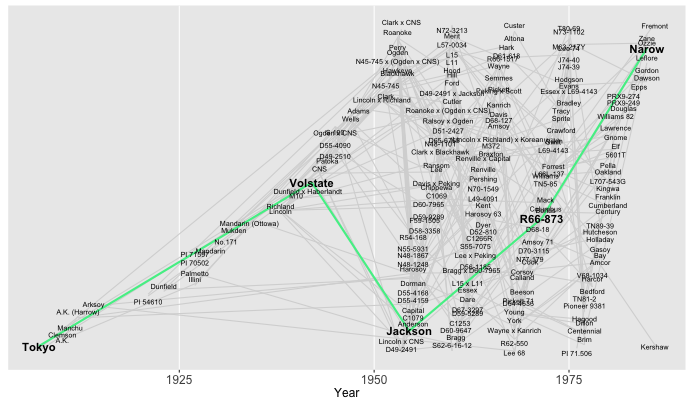
\includegraphics[width=\textwidth]{plotTNBin6}
    \end{framed}
    \caption{The shortest path between Tokyo and Narow, superimposed over the data structure, using a bin size of 6.}
    \label{fig:plotTNBin6}
\end{figure}

We can immediately see that Figure \ref{fig:plotTNBin6} more successfully mitigates text overlap compared to Figure \ref{fig:plotTNBin3}. We can also confirm what we saw in the previous plot that indeed most varieties were released between 1950 and 1970, and any textual overlap is confined to this range of years.

\section{Plotting ancestors and descendants by generation}
\label{remedy}

The most novel visual function in \pkg{ggenealogy}, \code{plotAncDes()} allows users to view the ancestors and descendants of a given variety. The inputted variety is highlighted in the center of the plot, ancestors are displayed to the left of the center, and descendants are displayed to the right of the center. The further from the center that a variety is located, the more generations that variety is distanced from the centered variety of interest.

This particular \pkg{ggenealogy} tool is unique because most available genealogy and graph visualization software do not allow for repeated labels. It is a useful tool because, as was demonstrated in Figures \ref{fig:kinshipFig} and \ref{fig:Graph}, some genealogical datasets require repeated node labels if they are to be visualized by generation counts. Indeed, our example soybean genealogy is one such dataset.

To demonstrate this tool, we will create a plot of the ancestors and descendants of the variety \code{Lee}. We specify that the maximum number of ancestor and descendant generations are both 6, and that the text of the variety of interest is highlighted in blue:

\mybox{
\texttt{R> plotAncDes("Lee", sbGeneal, mAnc = 6, mDes = 6, vCol = "blue")}
}

This generates the top plot of Figure \ref{fig:Lee}. We notice that \code{Lee} has 3 generations of ancestors and 5 generations of descendants. We also notice that some varieties are repeated in the plot, which is a unique feature provided by \pkg{ggenealogy}. For example, the variety \code{5601T} is represented four times - once as a third generation descendant of \code{Lee}, once as a fourth generation descendant of \code{Lee}, and twice as a fifth generation descendant of \code{Lee}. The variety \code{5601T} was repeated multiple times because there are multiple paths between \code{Lee} and \code{5601T}. For explanation purposes, all paths between \code{Lee} and \code{5601T} were manually highlighted in blue.

\begin{figure}[H]
    \begin{framed}
    \centering
    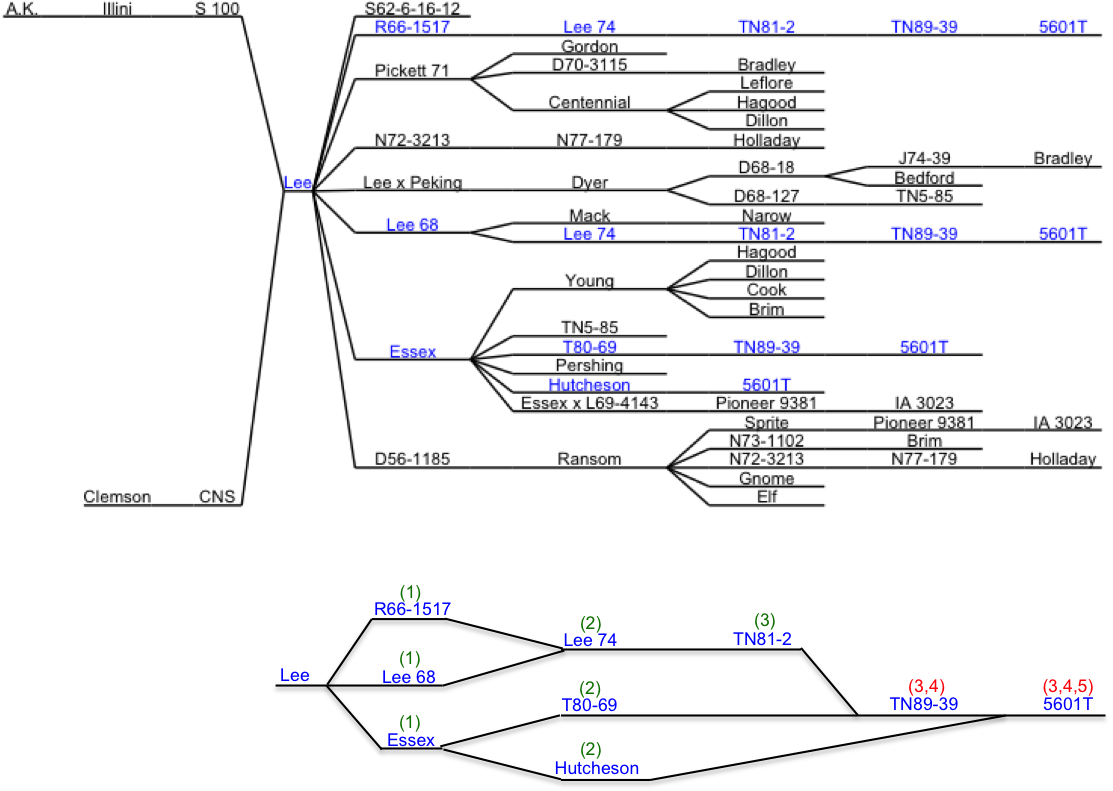
\includegraphics[width=\textwidth]{LeeAD3}
    \end{framed}
    \caption{Top: All ancestors and descendants of the variety Lee are shown in this ggenealogy plot. Bottom: We now attempt to mimic the blue paths in the ggenealogy plot on the top, only now nodes cannot be repeated. The parenthetical numbers above each node represents the set of generation counts that node is away from the center node Lee. The presence of red parentheses indicate that the plot on the bottom ambiguously display the example soybean genealogy in the way that the ggenealogy plot on the top can accomplish.}
    \label{fig:Lee}
\end{figure}

The bottom plot of Figure \ref{fig:Lee} is not an output plot of \pkg{ggenealogy}. Instead, it was simply created for didactic purposes. Here, the paths that were manually highlighted in blue in the top plot produced by \pkg{ggenealogy} are shown again, only now nodes cannot be repeated. The parenthetical number above each node represents the set of generation counts distancing that node from the center node \code{Lee}; green parentheses indicate that the node could be successfully placed in one horizontal position, but red parentheses indicate that the node could not be successfully placed in one horizontal position. We see that node \code{TN89-39} cannot simultaneously be represented as both a third and fourth descendent of node \code{Lee}, and node \code{5601T} cannot simultaneously be represented as a third, fourth, and fifth descendent of node \code{Lee}. Hence, without allowing nodes to repeat, this dataset cannot be presented in the graph on the bottom as it can be in the \pkg{ggenealogy} graph on the top. This is a current limitation in other genealogy and graphical software that \pkg{ggenealogy} can now provide.

\section{Plotting distance matrix}

It may also be of interest to generate matrices where the colors indicates a variable between all pairwise combinations of inputted varieties. The package \pkg{ggenealogy} also provides a function \code{plotDegMatrix()} for that purpose. We can demonstrate this function with the variable being the shortest path degree between a given pair of varieties. The shortest path degree is calculated as the smallest number of parent-child edges needed to traverse between two varieties of interest. For instance, in Figure \ref{fig:pathTNZB}, the shortest path degree between \code{Tokyo} and \code{Narow} is four and the shortest path degree between \code{Bedford} and \code{Zane} is ten.

Here we generate a distance matrix for a set of 10 varieties, setting the x-label and y-label as "Variety" and the legend label as "Degree". In this example, we add \pkg{ggplot2} functionality to specify that pairs with small degrees are white, while those with large degrees are dark green, as well as to specify the text size of the legend title and label.

\mybox{
\texttt{>R varieties <- c("Brim", "Bedford", "Calland", "Dillon", "Hood", "Narow", "Pella", "Tokyo", "Young", "Zane")}\\
\texttt{>R plotDegMatrix(varieties, sbIG, sbGeneal, "Variety", "Variety", "Degree") + ggplot2::scale\_fill\_continuous(low = "white", high = "darkgreen") + ggplot2::theme(legend.title = ggplot2::element\_text(size = 15), legend.text = ggplot2::element\_text(size = 15))}
}

This creates the plot in Figure \ref{fig:degMatrix}. We see that the degree of the shortest path between varieties \code{Bedford} and \code{Zane} is 10, which is consistent with what we saw earlier in Figure \ref{fig:pathTNZB}. However, we now also see that a shortest path degree of 10 may be considered relative to the rest of this dataset.

\begin{figure}[h]
    \begin{framed}
    \centering
    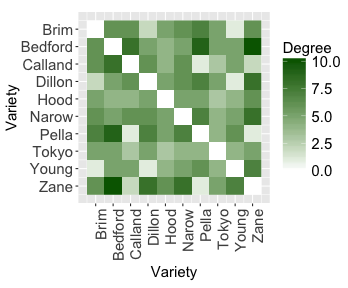
\includegraphics[width=0.5\textwidth]{degMatrix}
    \end{framed}
    \caption{The shortest path degree matrix between ten varieties of interest.}
    \label{fig:degMatrix}
\end{figure}

\section{Academic genealogy of statisticians}

The \pkg{ggenealogy} package comes with two example datasets, and while we have introduced the plant breeding genealogy, we have yet to introduce the academic genealogy. As was demonstrated in Section \ref{exData}, every parent in the academic genealogy is also a child, and some children in the academic genealogy have more than two parents. Neither of these features was the case in the plant breeding genealogy. Additionally, the academic genealogy is much larger than the plant breeding genealogy. Some of these differences may affect how one would approach \pkg{ggenealogy} plotting tools. For this reason, we will now demonstrate some of the \pkg{ggenealogy} plotting tools we already introduced, only now applied to the academic genealogy. 

The ability to plot ancestors and descendants by generation was demonstrated using the plant breeding genealogy in Figure \ref{fig:Lee}. As we believe this is the most novel plotting tool in the \pkg{ggenealogy} package, we will test it again here using the academic genealogy.

We need to choose a central individual of interest in order to create this plot. Perhaps we can use the academic statistician in the dataset that has the largest number of "descendants". To determine the name of this individual, below we use the \pkg{ggenealogy} function \code{getNode()} to create a vector \code{indVec} that contains the names of all individuals in the dataset. We then use the \pkg{dplyr} package to apply the \pkg{ggenealogy} function \code{getDescendants()} on each individual in the \code{indVec} vector (\citealt{dplyr}). We set the parameter \code{gen} to a conservatively large value of 100 as this dataset is unlikely to have any individuals with more than 100 generations of "descendants".

After that, we can generate a table to examine all values of "descendant" counts in the dataset, along with the number of individuals who have each of those values of "descendant" counts. Of the 8165 individuals in this dataset, 6252 of them have zero "descendants", 322 of them have one "descendant", and 145 of them have two "descendants". There are only 17 individuals who have more than 30 "descendants", and there is one individual who has the largest value of 159 "descendants". We determine that this individual is the prominent British statistician Sir David Cox, who is known for the Box-Cox transformation and Cox processes, as well as for mentoring many younger researchers who later became notable statisticians themselves.

\mybox{
\texttt{>R library(dplyr)}\\
\texttt{>R indVec <- getNodes(statGeneal)}\\
\texttt{>R indVec <- indVec[which(indVec != "", )]}\\
\texttt{>R dFunc <- function(var) nrow(getDescendants(var, statGeneal, gen = 100))}\\
\texttt{>R numDesc <- sapply(indVec, dFunc)}\\
\texttt{>R table(numDesc)}
}

\mybox[green!10]{
\texttt{numDesc}\\
\texttt{   0    1    2    3    4    5    6    7    8    9   10   11   12   13   14 }\\
\texttt{6252  322  145   88   58   36   31   22   23   14   17   13   14    9    9 }\\
\texttt{  15   16   17   18   19   20   21   22   23   24   25   26   27   29   30 }\\
\texttt{   6    4    3    2    5    7    5    3    3    2    2    6    1    1    3 }\\
\texttt{  34   37   38   40   41   44   45   48   49   61   62   75   77   84  159 }\\
\texttt{   2    1    1    1    1    1    1    1    2    1    1    1    1    1    1 }
}

\mybox{
\texttt{R> which(numDesc == 159)}
}

\mybox[green!10]{
\texttt{David Cox}\\ 
\texttt{     1980}
}

We can now visualize how these 159 "descendants" are related to Sir David Cox by calling the \code{plotAncDes()} function of \pkg{ggenealogy}, similar to what we did to generate Figure \ref{fig:Lee}. As such, we create Figure \ref{fig:dCox} using the code below.

\mybox{
\texttt{R> plotAncDes("David Cox", statGeneal, mAnc = 6, mDes = 6, vCol = "blue")}
}

\begin{figure}%[h]
    \begin{framed}
    \centering
    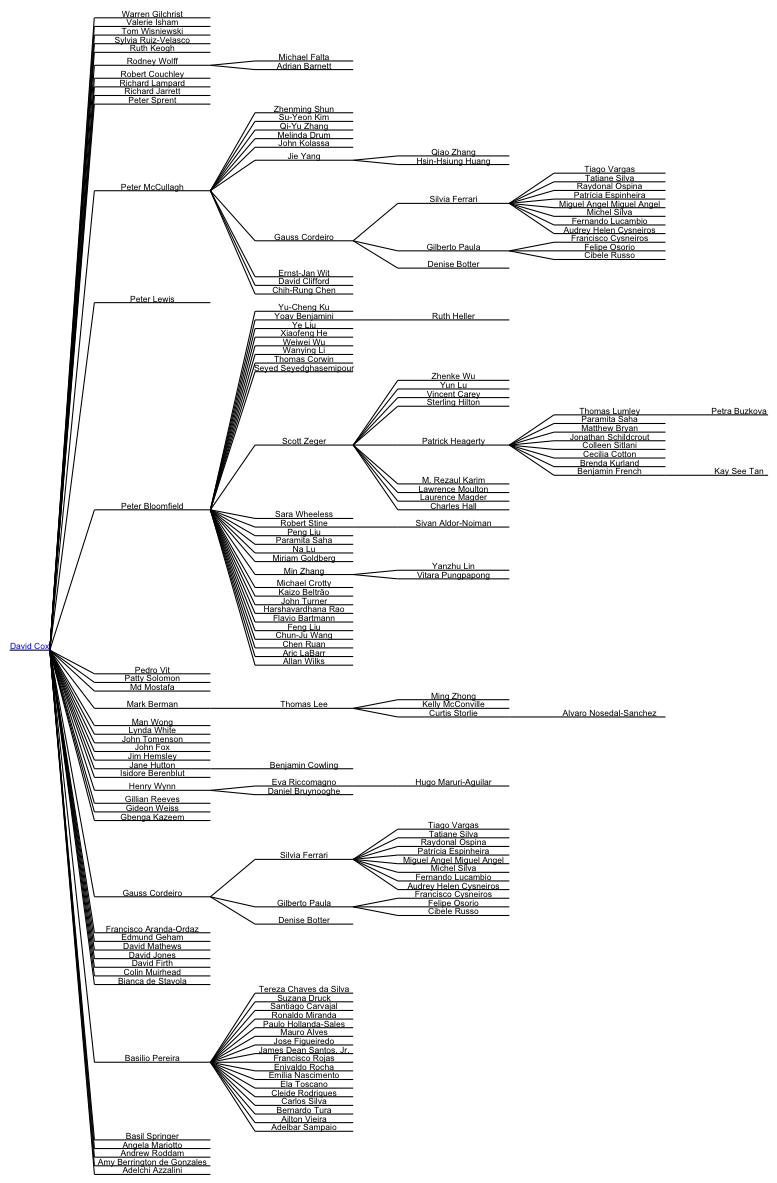
\includegraphics[width=\textwidth]{dCox.png}
    \end{framed}
    \caption{The 159 academic statistician "descendants" of Sir David Cox.}
    \label{fig:dCox}
\end{figure}

We see from Figure \ref{fig:dCox} that Sir David Cox had 42 "children", many of them becoming notable statisticians themselves, such as Basilio Pereira, Valerie Isham, Gauss Cordeiro, Peter McCullagh, and Henry Wynn. Of his "children", the one who produced the most "children" of their own was Peter Bloomfield, who has 26 "children" and 49 "descendants". In total, Sir David Cox had five generations of academic statistics mentees in this dataset.

\mybox{
\texttt{R> length(getChild("Peter Bloomfield", statGeneal))}
}

\mybox[green!10]{
\texttt{[1] 26}
}

\mybox{
\texttt{R> nrow(getDescendants("Peter Bloomfield", statGeneal, gen = 100))}
}

\mybox[green!10]{
\texttt{[1] 49}
}

At this point, it would be insightful to examine a more detailed view of one of the longest strings of "parent-child" relationships between Sir David Cox and one of the two individuals who are his fifth generation "descendants". We do so with the code below, choosing his fifth generation "descendant" to be Petra Buzkova. We set the \code{fontFace} variable of the \code{plotPath()} to a value of 4, indicating we wish to boldface and italicize the two varieties of interest.

\mybox{
\texttt{R> statIG <- dfToIG(statGeneal)}\\
\texttt{R> pathCB <- getPath("David Cox", "Petra Buzkova", statIG, statGeneal, isDirected = FALSE)}\\
\texttt{R> plotPath(pathCB, fontFace = 4) + ggplot2::theme(axis.text = ggplot2::element\_text(size = 10), axis.title = ggplot2::element\_text(size = 10))}
}

\clearpage

\begin{figure}[H]
    \begin{framed}
    \centering
    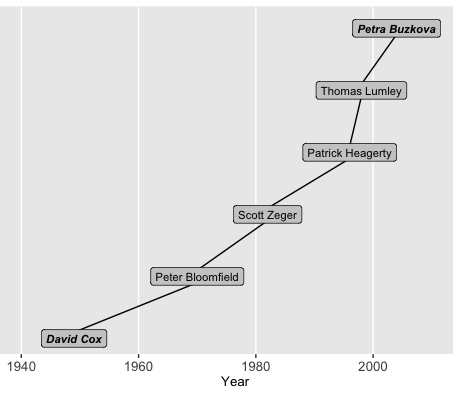
\includegraphics[width=0.7\textwidth]{pathCB}
    \end{framed}
    \caption{The shortest path between Sir David Cox and one of his fifth generation "descendants", Petra Buzkova.}
    \label{fig:pathCB}
\end{figure}

This code results in Figure \ref{fig:pathCB}. We see that the shortest path between Sir David Cox and Petra Buzkova is strictly composed of five unidirectional "parent-child" relationships that span about 55 years. We see that the time difference between when an advisor and student earned their degrees is not consistent across this path: The three statisticians who earned their degrees earliest in this path span more than 30 years in degree acquisition, whereas the three statisticians who earned their degrees later in this path only span less than ten years in degree acquisition.

We also notice in Figure \ref{fig:pathCB} that Sir David Cox received his statistics degree in about 1950, and Petra Buzkova received her statistics degree in about 2005. This genealogy only contains historical information about obtained degrees, and does not project into the future. Hence, we can be assured that Petra Buzkova is one of the younger individuals in the dataset, at least in the sense that the youngest individual could only have received his or her degree ten years after Petra Buzkova. However, we cannot be assured that Sir David Cox is one of the oldest individuals in the dataset. As such, it would be informative to superimpose this path of interest onto the entire dataset, using the \code{plotPathOnAll()} function of the \pkg{ggenealogy} package, as we did for the soybean genealogy in Figures \ref{fig:plotTNBin3} and \ref{fig:plotTNBin6}.

We can achieve this using the below code. After trial and error, we use a \code{binVector} of size 200, and append \pkg{ggplot2} syntax to define suitable x-axis limits. The output of this process is illustrated in Figure \ref{fig:plotCBText}.

\mybox{
\texttt{R> plotPathOnAll(pathCB, statGeneal, statIG, binVector = 1:200) + ggplot2::theme(axis.text = ggplot2::element\_text(size = 8), axis.title = ggplot2::element\_text(size = 8)) + ggplot2::scale\_x\_continuous(expand = c(.1, .2))}
}

\begin{figure}[H]
    \begin{framed}
    \centering
    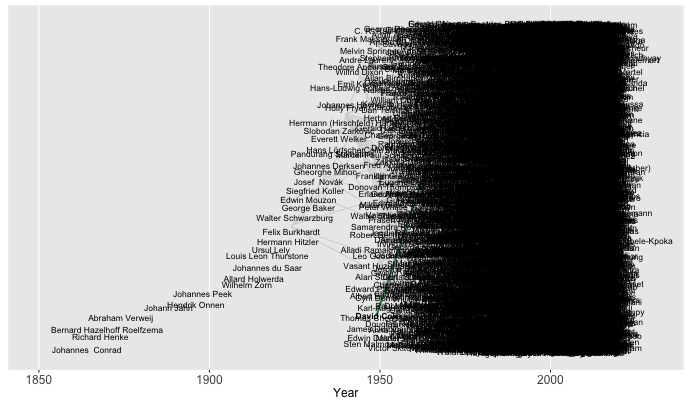
\includegraphics[width=\textwidth]{plotCBText}
    \end{framed}
    \caption{The shortest path between Sir David Cox and Petra Buzkova, superimposed over the data structure, using a bin size of 200.}
    \label{fig:plotCBText}
\end{figure}

We see from the resulting Figure \ref{fig:plotCBText} that almost all text labels for individuals who received their graduate-level statistics degrees between 1950 and 2015 are undecipherable. We also see that the year Sir David Cox acquired his statistics degree is somewhere in the later half of the variable year for this dataset, as the oldest dates for acquisition of statistics degrees in this dataset occur around 1860. However, the number of individuals who are documented as receiving their statistics degrees between 1860 and 1950 are few enough so that their text labels are somewhat readable.

The text labels are so numerous in Figure \ref{fig:plotCBText} that simply trying different values for the input parameter \code{binVector} will not solve the text overlapping problem. Instead, one approach we can try is to reconstruct the plot using the same \pkg{ggenealogy} function \code{plotPathOnAll()}, only now specifying variables to render the size (2.5) and color (default of black) of the text for nodes that are on the path of interest to be more noticeable than the size (0.5) and color (dark gray) of the text for nodes that are not on the path of interest. Moreover, we can make the edges that are not on the path of interest to be represented in a less noticeable color (light gray) than the edges that are on the path of interest (default of dark green). The variable names and options for these aesthetics is further detailed in the help manual of the function. We provide one example code that alters the defaults of the text color and sizes of nodes and edges below, which results in Figure \ref{fig:plotCBNoText}.

\mybox{
\texttt{R> plotPathOnAll(pathCB, statGeneal, statIG, binVector = 1:200, nodeSize = .5, pathNodeSize = 2.5, nodeCol = "darkgray", edgeCol = "lightgray") + ggplot2::theme(axis.text = ggplot2::element\_text(size = 8), axis.title = ggplot2::element\_text(size = 8)) + ggplot2::scale\_x\_continuous(expand = c(.1, .2))}
}

\begin{figure}[H]
    \begin{framed}
    \centering
    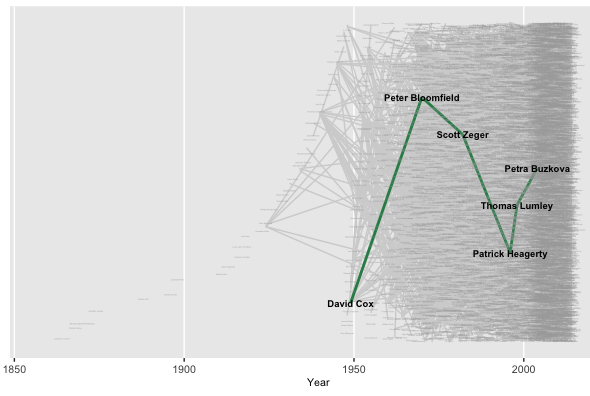
\includegraphics[width=\textwidth]{plotCBNoText}
    \end{framed}
    \caption{The shortest path between Sir David Cox and Petra Buzkova, superimposed over the data structure, using a bin size of 200. Individuals on the shortest path are labeled in large and black text and connected by dark green edges; all other individuals are labeled in small and gray text and connected by light gray edges.}
    \label{fig:plotCBNoText}
\end{figure}

In Figure \ref{fig:plotCBNoText}, we can now see each individual on the path of interest, and how their values for the variable year are overlaid on the entire genealogy structure. We can also more clearly see that, even though only ten years span between the youngest individual in the genealogy and Petra Buzkova, there are many individuals in that last decade. Indeed, the decade from 2005 to 2015 appears to be the densest in this dataset in terms of acquisition of statistics degrees.

\subsection{Interactive visualization of genealogical structure}

We could still improve upon Figure \ref{fig:plotCBNoText}. Even though we may be primarily interested in understanding how the path of interest is overlaid across the entire genealogical structure, we could, upon viewing the entire structure, also develop an interest in nodes that are not on the path of interest but are revealed to stand out among the rest of the genealogical structure. For instance, in Figure \ref{fig:plotCBNoText}, it may be of interest for us to determine the names of the few individuals who obtained their statistics degrees before 1900. Fortunately, within the \code{plotPathOnAll()} function, there is a variable \code{animate} that we can set to a value of TRUE to create an interactive version of the figure that allows us to hover over individual illegible labels and immediately receive their labels in a readable format. A short video demonstration of these interactive features can be viewed upon clicking on Figure \ref{fig:plotAnimate}.

\mybox{
\texttt{R> plotPathOnAll(pathCB, statGeneal, statIG, binVector = 1:200, nodeSize = .5, pathNodeSize = 2.5, nodeCol = "darkgray", edgeCol = "lightgray", animate = TRUE)}
}

\clearpage

\begin{figure}[H]
    \begin{framed}
    \centering
    \includemedia[width=1.0\textwidth, addresource=animateGen.mov, deactivate=onclick, flashvars={source=animateGen.mov}]{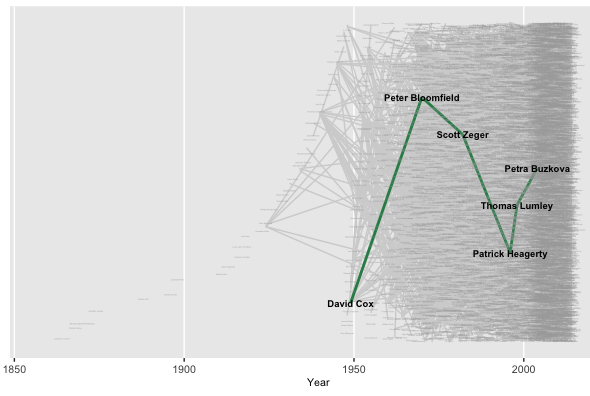
\includegraphics{./plotCBNoText.png}}{VPlayer.swf}
    \end{framed}
    \caption{Upon clicking on this figure twice, a short video demonstrating the animation features for this function can be viewed. Please note that to properly view this video, the PDF version of this paper must be opened in Adobe Acrobat Reader DC (Version >=9), which can be downloaded free of charge.}
    \label{fig:plotAnimate}
\end{figure}

\section{Future avenues}

We have several avenues we could pursue to expand upon this work:

\begin{enumerate}
\item \textbf{Incorporation of the Shiny application}: The reactive programming could save users of \pkg{ggenealogy} the time of using command line for each change of input as well as the inefficiency of rerunning code. It could also enhance the interactivity. A Shiny application that uses certain \pkg{ggenealogy} functionality is already available for users who wish to explore the soybean genealogy; the data can be viewed at \url{http://shiny.soybase.org/CNV/}.

\item \textbf{Expanding on variable types}: We could incorporate plotting tools that examine not only quantitative variables (such as our example variable of "year"), but also categorical variables associated with individuals in datasets.

\item \textbf{Further eliminate text overlap}: The \pkg{ggenealogy} visualization tool \code{plotPathOnAll()} is suitable as a data exploration tool, but not always as a publication tool. This is because we still see textual overlap in datasets that are small enough to - in theory - be represented with all labels in a readable format (see Figure \ref{fig:plotTNBin6}). As such, we plan to add a feature to the package that allows users to manually fine-tune automated plots. For example, after comparing several bin sizes on the soybean genealogy, we determined that the bin size of 6 produced the minimal textual overlap, as is seen in Figure \ref{fig:plotTNBin6}. If we could subsequently fine-tune the vertical positions of the small fraction of text labels that remained overlapped after the automated \pkg{ggenealogy} function, then we could potentially remove all overlaps, and the plot could be used in presentations and publications.

\item \textbf{Test on additional datasets}: We look forward to testing the \pkg{ggenealogy} package on additional genealogical data sets. Exploring several datasets with the software will allow us to fix remaining bugs, and provide us further insight into how to make our tools available for a wide range of data input formats. 
\end{enumerate}

\section{Conclusions}

The \pkg{ggenealogy} package offers various plotting tools that can assist those studying genealogical lineages in the data exploration phases, as well as in preparing publication-suitable images. As each plot comes with its pros and cons, we recommended for users to explore several visualization tools. If users are simultaneously using similar packages, we in particular recommend using the \code{plotAncDes()} function. This plot allows users to view generation counts of a variety of interest in a manner that is not as readily available in similar software packages.

\section{Acknowledgments}

This project was an effort between Susan VanderPlas, Dianne Cook, Michelle A. Graham, and myself. Together, we  thank Drs. James E. Specht and Randy C. Shoemaker for helpful discussions of soybean genealogy. In addition, we are grateful for the financial support from the United Soybean Board (Project 1204), The North Central Soybean Research Program, the NSF Plant Genome Research Program (award number 0820642), and the USDA-ARS CRIS Project 3625-21220-005-00D. The USDA is an equal opportunity provider and employer. Mention of trade names or commercial products in this article is solely for the purpose of providing specific information and does not imply recommendation or endorsement by the U.S. Department of Agriculture.










%%%%%%%%%%%%%%%%%%%%%%%%%%%%%%%%%%%%%% CHAPTER %%%%%%%%%%%%%%%%%%%%%%%%%%%%%%%%%%%%%% 
%%%%%%%%%%%%%%%%%%%%%%%%%%%%%%%%%%%%%%%%%%%%%%%%%%%%%%%%%%%%%%%%%%%%%%%%%%%%%%%%%%%%%

\chapter{The case for visualization methods in RNA-sequencing data analysis}
\label{sec:clustering}

\section{Introduction}

RNA-sequencing (RNA-seq) uses next-generation sequencing (NGS) to estimate the quantity of RNA in biological samples at given timepoints. In recent years, decreasing cost and increasing throughput has rendered RNA-seq an attractive alternative to transcriptome profiling. Prior to RNA-seq, gene expression studies were performed with microarray techniques, which required prior knowledge of reference sequences. RNA-seq does not have this limitation, and has enabled a new range of applications such as transcriptome de novo assembly \citep{Robertson} and detection of alternative splicing processes \citep{Anders2012, Pan}. Coupled with its high resolution and sensitivity, RNA-seq will likely revolutionize our understanding of the intricacies of eukaryotic transcriptomes \citep{Wang, Zhao}.

RNA-seq data is multivariate data, and its basic form is a matrix containing mapped read counts for \textit{n} rows of genes and \textit{p} columns of samples. These mapped read counts provide estimations of the gene expression levels across samples. Researchers typically conduct RNA-seq studies to identify differentially expressed genes (DEGs) between treatment groups. In most popular RNA-seq analysis packages, this objective is approached with models, such as the negative binomial model \citep{Anders2010, Trapnell2012, Trapnell2013, Robinson} and linear regression models \citep{Law}.

Initially, it was widely claimed that RNA-seq produced unbiased data that did not require sophisticated normalization \citep{Wang, Morin, Marioni}. However, numerous studies have since revealed that RNA-seq data is replete with biases and that accurate detection of DEGs is not a negligible task. Problems that complicate the analysis of RNA-seq data include nucleotide and read-position biases \citep{Hansen}, biases related to gene lengths and sequencing depths \citep{Oshlack, RobinsonOshlack}, biases introduced during library preparation \citep{McIntyre}, biases pertaining to the number of replications \citep{Schurch}, biases derived from overlapping sense-antisense transcripts and gene isoforms \citep{Trapnell2013}, and the confounding combination of technical and biological variability \citep{Bullard}.

In light of these complications, researchers should analyze RNA-seq data like they would any other biased multivariate data. Simply applying models to such data is problematic because models hold assumptions that they alone cannot call into question. Fortunately, data visualization enables researchers to see patterns and problems they may not otherwise detect with traditional modeling. As a result, the most effective approach to data analysis is to iterate between models and visuals, and enhance the appropriateness of applied models based on feedback from visuals \citep{Shneiderman}. With RNA-seq data, we primarily want to compare the variability between replicates and between treatment groups. This is visually best achieved by drawing the mapped read count distributions across all genes and samples. Unfortunately, the few plotting tools offered in popular RNA-seq packages do not allow users to effectively view their data in this manner.

In this paper, we strive to remedy this problem by publishing new and effective RNA-seq plotting tools. We use real RNA-seq data to show that our tools can detect normalization problems, DEG designation problems, and common errors in the analysis pipeline. We also show that our tools can identify genes of interest that cannot otherwise be obtained by models. We emphasize that interactive graphics should be an indisposable component of modern RNA-seq analysis: Researchers should be able to quickly flip through plots of genes that appear promising or problematic, and link between plots to swiftly obtain various perspectives of their data. Here, we do not propose that users drastically change their approach to RNA-seq analysis. Instead, we propose that users simply modify their approach to RNA-seq analysis by assessing the sensibility of their models with multivariate graphical tools, namely with parallel coordinate plots, scatterplot matrices, and litre plots.

\section{Parallel Coordinate Plots}

Parallel coordinate plots are essential to visually verify the relationships between variables in multivariate data. A parallel coordinate plot draws each row (gene) as a line. Connections between samples with positive correlations are flat, and connections between samples with negative correlations are crossed. The ideal dataset has more variability between treatments than between replicates. Researchers can quickly confirm this with a parallel coordinate plot: There should be flat connections between replicates but crossed connections between treatments.

There are several packages within the Bioconductor software that provide graphics for RNA-seq data analysis \citep{Huber}. Two of the most common graphic techniques are side-by-side boxplots and Multidimensional Scaling (MDS) plots \citep{Love, Risso, Robinson, Ritchie}. Unfortunately, these plots can hide problems that still exist in the data even after normalization and that could be better detected with parallel coordinate plots.

Figure~\ref{simulatedData} exemplifies this problem for two simulated datasets, one displayed on the left half and the other displayed on the right half of the figure. Each dataset contains two treatment groups (A and B) with three replicates. We cannot detect any notable differences between the left and right datasets from the side-by-side boxplots (subplots A) as they both show fairly consistent five number summaries across their six samples. Likewise, we cannot detect notable differences between the datasets from the MDS plots (subplots B) as they both suggest that the datasets are clustered by the two treatment groups, although the first replicate from treatment A appears as an outlier in the right MDS plot.

\begin{figure}[!tpb]
\centerline{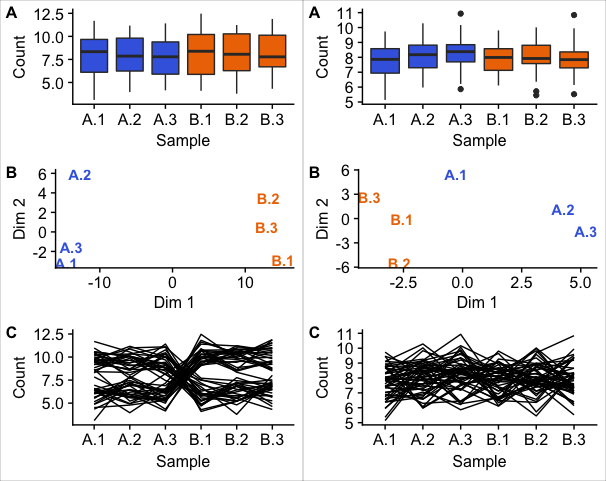
\includegraphics[width=\columnwidth]{MakeFigures/simulatedData.jpg}}
\caption{One simulated dataset is shown on the left half and another simulated dataset is shown on the right half of the figure. We do not see crucial distinctions between the left and right datasets when we compare their boxplots (A subplots) and MDS plots (B subplots). However, their parallel coordinate plots (C subplots) show a critical difference between their structures. Namely, the left dataset is composed of genes with small replicate variation and large treatment group variation (suggesting DEGs), while the right dataset is composed of genes with similar variation between replicates and treatment groups (not suggesting DEGs). 
\label{simulatedData}}
\end{figure}

Despite this, we immediately see from the parallel coordinate plots (subplots C) that the left and right datasets have an important difference. The left dataset has consistent (level) lines between replicates and inconsistent (crossed) lines between treatment groups. This suggests that some of the genes (lines) have consistently low values for treatment group A and consistently high values for treatment group B, while some genes have the opposite phenomenon. As a result, these plotted genes are likely candidates for differential expression. In contrast, the right dataset does not possess this ideal structure and suggests that the genes may not be candidates for differential expression. We could not see this important distinction using the side-by-side boxplots or the MDS plots because they only provide data summarization at the sample resolution, while the parallel coordinate plots show the sample connections for each of the 50 genes.

We will now examine the application of parallel coordinate plots to data from an RNA-seq study that compared soybean leaves in iron-sufficient (group P) and iron-deficient (group N) soil conditions \citep{Lauter16}. We filtered genes with low means and/or variance, performed a hierarchical clustering analysis with a cluster size of four, retained only significant genes, and visualized the results using parallel coordinate lines (Figure~\ref{sbIRClustersSig}). To view the results before the non-significant genes were removed, see Supplementary Figure 1. For these visualizations, we standardized each gene to have a mean of zero and standard deviation of unity \citep{Chandrasekhar, deSouto}.

The majority of significant genes were in Clusters 1 and 2, which for the most part captured the expected patterns of differential expression (consistent replicates and inconsistent treatments) in mirroring ways. Only 17 significant genes belonged to Cluster 4 and they mostly showed messy patterns with low signal to noise ratios. Interestingly, Cluster 3 had a fairly large number of significant genes (n=861). These genes mostly showed clean differential expression profiles similar to Cluster 2 (large values for group N and small values for group P), except for unexpectedly large values for the third replicate of group P. The reasons for a different response by these genes on this replicate is unclear, but warrants further study.

\begin{figure}[!tpb]
\centerline{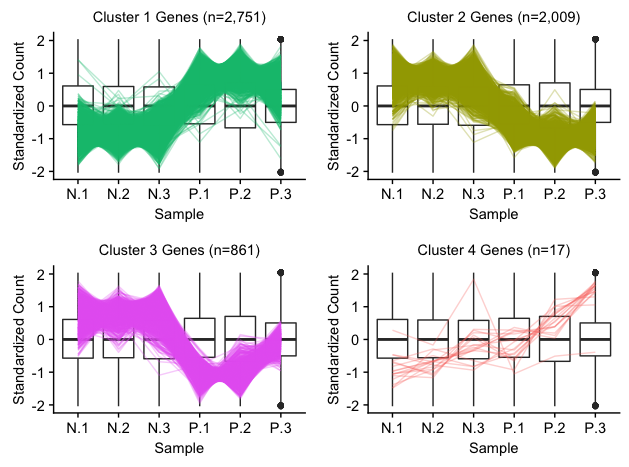
\includegraphics[width=\columnwidth]{MakeFigures/sbIRClustersSig.jpg}}
\caption{Using parallel coordinate plots to visualize significant genes after hierarchical clustering. We can quickly confirm that Clusters 1 and 2 show the typical pattern for significant genes. Cluster 4 does not distinctively show the usual profile for significant genes. Cluster 3 looks similar to Cluster 2, except for unexpectedly large P.3 values.
\label{sbIRClustersSig}}
\end{figure}

\section{Scatterplot matrices}

\subsection{Overview of scatterplot matrices}

A scatterplot matrix is another effective multivariate visualization tool that plots the mapped read count distributions across all genes and samples. Specifically, it represents each row (gene) as a point in each scatterplot. With this method, users can quickly discover unexpected patterns, recognize geometric shapes, and assess the structure and association between multiple variables in a manner that is different from most common practices. 

Clean data would be expected to have larger variability between treatment groups than between replicates. As Figure~\ref{sbIRClustersSig} shows, researchers can quickly confirm this with a scatterplot matrix. Within each scatterplot, most genes should fall along the \textit{x=y} line (in red) as we expect only a small proportion of them to show differential expression between samples. However, a fraction of the genes should have lower variability between replicates than between treatments, and so we should expect the spread of the scatterplot points to fall more closely along the \textit{x=y} relationship between replicates than between treatments. Indeed, in Figure~\ref{sbIRClustersSig}, we created a scatterplot matrix for a public RNA-seq dataset that contains three replicates for two developmental stages of soybean cotyledon (S1 and S2) \citep{Brown}. We can immediately verify that the nine scatterplots between treatment pairs (in the bottom-left corner of the matrix) have more spread around the \textit{x=y} line than the six scatterplots between replicate pairs.

\begin{figure}[!tpb]
\centerline{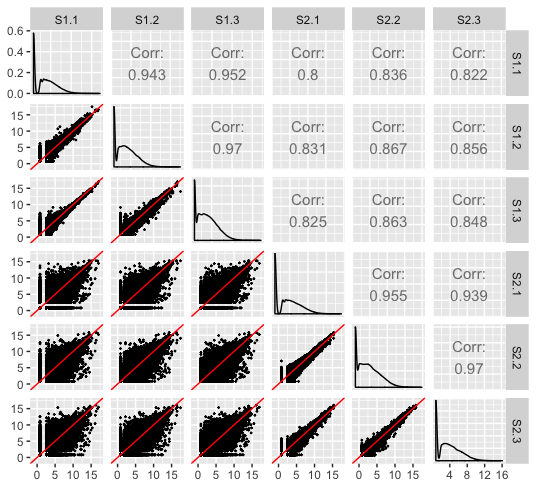
\includegraphics[width=\columnwidth]{MakeFigures/sbCNSM.jpg}}
\caption{Example of the expected structure of an RNA-seq dataset, using soybean cotyledon data from \cite{Brown}. Within a given scatterplot, most genes (points) should fall along the \textit{x=y} line. We should see genes deviate more strongly from the \textit{x=y} line in treatment scatterplots than in replicate scatterplots. 
\label{sbCNSM}}
\end{figure}

After confirming this expected trend, users can use the scatterplot matrix to focus on subsets of genes: Outlier genes that deviate from the \textit{x=y} line in replicate scatterplots might be problematic, whereas outlier genes that deviate from the \textit{x=y} line in treatment scatterplots might be DEGs. In order to achieve this functionality, the plots must be rendered interactive.

Notice that each gene in our data is plotted once in each of the 15 scatterplots. With 73,320 genes in our data, more than one million points must be plotted. Rendering all points interactive would slow down the interactive capabilities of the plot. To solve this, we can tailor the geometric object of the scatterplots to be hexagon bins rather than points. This dramatically reduces the number of geometric objects to be plotted, and increases the interactivity speed.

The reader can visit https://rnaseqvisualization.shinyapps.io/scatmat to access the interactive version of Figure~\ref{sbIRClustersSig}. Readers can read the ``About" Tab to fully understand how to use the application. Essentially, the user can hover over a hexagon bin to see how many genes it contains. When the user clicks on a hexagon bin, the names of the genes are listed and superimposed as orange points across all scatterplots. The genes are also linked to a second plot that superimposes them as parallel coordinate lines on a side-by-side boxplot of all gene counts. This interactivity and linking allows users to quickly examine genes of interest from multiple perspectives superimposed onto the summary of all genes in the dataset. 

\subsection{Assessing normalization with scatterplot matrices}

There is still substantial discussion about the normalization of RNA-seq data, and the scatterplot matrix can be used to understand and assess various algorithms. To exemplify this point, we will use a publicly-available RNA-seq dataset on Saccharomyces cerevisiae (yeast) grown in YP-Glucose (YPD) \citep{Risso}. The data contained four cultures from independent libraries that were sequenced using two library preparation protocols and either one or two lanes in a total of three flow-cells. This experimental design allowed researchers to examine various levels and combinations of technical effects (library preparation and protocol and flow cell) and biological effects (culture).

The four cultures (Y1, Y2, Y4, and Y7) were treated as biological replicates for which differential expression was not expected. Hence, the authors could establish a false positive rate in relation to the number of DEGs called between these groups. They then demonstrated that within-lane regression alone was insufficient in effectively removing biases. Instead, aggressive corrections for both within-lane (GC-content and gene length) and between-lane (count distribution and sequencing depth) biases were needed to effectively reduce the false-positive rate of differential expression calls.

Figure~\ref{yeastWithinBetween}A shows the scatterplot matrix of the read counts from the Y1 and Y4 treatments after within-lane normalization. As we stated earlier, we expect most genes to show similar expression between samples, except for the handful that are differentially expressed. However, it is immediately clear that the data still was not sufficiently normalized as the distribution of genes is not centered around the \textit{x=y} lines. In contrast, Figure~\ref{yeastWithinBetween}B shows the scatterplot matrix of the read counts from the Y1 and Y4 treatments after \textit{both} within-lane and between-lane normalization, as was recommended by the authors due to its reduced false-positive rate. Indeed, the scatterplot matrix now follows the expected structure with most genes falling along the \textit{x=y} line with thicker deviations from it between treatment groups than between replicate groups.

Additionally, we can also confirm from Figure~\ref{yeastWithinBetween}B that the read counts fall closer to the \textit{x=y} line between the Y4 replicates (bottom-right scatterplot) than between the Y1 replicates (top-left scatterplot). This is expected because the Y1 replicates had additional technical variability as they used two different flow cells, whereas the Y4 replicates were from the same flow cell. As such, the scatterplot matrix can also be used to quickly inspect patterns of biological and technical variability in the dataset.

\subsection{Checking for common errors with scatterplot matrices}

Irreproducibility is prevalent in high-throughput biological studies. A study in Nature Genetics surveyed eighteen published microarray expression analyses and reported that only two were exactly reproducible \citep{Ioannidis}. The extent of the problem has spawned a field called ``forensic bioinformatics" whereby researchers attempt to reverse-engineer reported results back into the raw datasets simply to derive the methodologies used in published studies \citep{Baggerly}.

\begin{figure}[!tpb]
\centerline{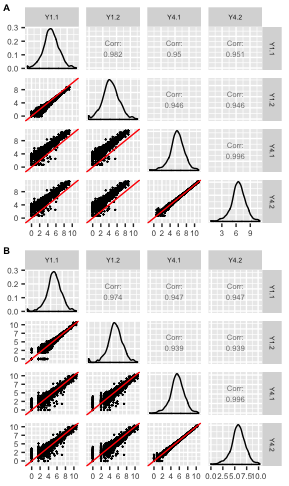
\includegraphics[width=\columnwidth]{MakeFigures/yeastWithinBetween.jpg}}
\caption{Illustrating normalization checks with data from  \cite{Risso}. The collective deviation of genes from the \textit{x=y} line instantly reveals that the RNA-seq dataset was not thoroughly normalized using within-lane normalization (subplot A). However, within-lane normalization followed by between-lane normalization sufficiently normalized the data (subplot B). The authors who developed these normalization methods showed that the later approach generated a lower false-positive DEG call rate in this dataset.
\label{yeastWithinBetween}}
\end{figure}

Even though irreproducibility is merely cumbersome when it masks methods, it is unquestionably hazardous when it masks errors. With regards to personalized medicine, for example, obscured errors may cause well-intentioned researchers to present evidence for drugs that are ineffective or even harmful to patients \citep{Baggerly}. Forensic bioinformaticians who have actively investigated common errors in high-throughput biological studies have concluded that the largeness of the data itself may hinder our ability to detect errors \citep{Baggerly}. They also discovered that the most common errors are simple errors, such as mixing up sample labels \citep{Baggerly}. Collectively, these findings suggest that simple errors can be difficult to detect using common practices in high-throughput studies.

Fortunately, scatterplot matrices are a simple tool to check for common errors like sample mislabeling. Figure~\ref{sbCNSwitchedSM} shows the resulting scatterplot matrix after we deliberately swapped the labels of the third replicate of the first treatment group (S1.3) with the first replicate of the second treatment group (S2.1) in the previously-mentioned cotyledon dataset. We can immediately see that, as expected, there are nine scatterplots with thicker distributions around the \textit{x=y} line and six scatterplots with thinner distributions around the \textit{x=y} line. However, we notice that a subset of these thick and thin scatterplots appear outside of their expected locations given the expected variability between treatments versus replicates. Rearranging the columns of the two samples that appear suspicious in Figure~\ref{sbCNSwitchedSM} would indeed lead us back to the clean-looking scatterplot matrix we saw in Figure~\ref{sbIRClustersSig}. We cannot detect this mislabeling problem as convincingly with traditional plots, as can be verified with this dataset by comparing the boxplots and MDS plots before sample switching (left side of Supplementary Figure 6) and after sample switching (right side of Supplementary Figure 6). 


\subsection{Finding unexpected patterns in scatterplot matrices}

Most popular RNA-seq plotting tools display summaries about the read counts, such as fold change summaries, principal component summaries, five number summaries, and dispersion summaries. In contrast to this trend, scatterplot matrices display the non-summarized read counts for all genes. This trait allows for geometric shapes and patterns relevant to the read count distribution to be readily visible in the scatterplot matrix.

An example of how geometric shapes in the scatterplot matrix can provide applicable information to researchers is shown in Figure~\ref{structure}, which uses the iron-metabolism soybean dataset \citep{Lauter16}. After normalizing the data, we see the expected pattern of a scatterplot matrix, with more variation around the \textit{x=y} line between treatments than between replicates (Figure~\ref{structure}). 

%%%%%%%%%%%%%% Ask Michelle for thoughts below %%%%%%%%%%%%%%%%%%%
However, one streak structure in the bottom right scatterplot stands out. A small subset of transcripts between replicates of the iron-sufficient group sharply deviates from the \textit{x=y} line. By interacting with the plot, we determined the identification of the five transcripts that deviated the most from the expected pattern, and searched for their putative functions. We discovered that these transcripts are reportedly involved in biotic and abiotic stress responses as well as the production of superoxides to combat microbial infections. This is the same group of genes discussed in Figure~\ref{sbIRClustersSig}. It should be noted that these five transcripts did not reach significance unless the third replicate of the P group was removed. In any case, we would not have observed this interesting structure from any models.

\begin{figure}[!tpb]
\centerline{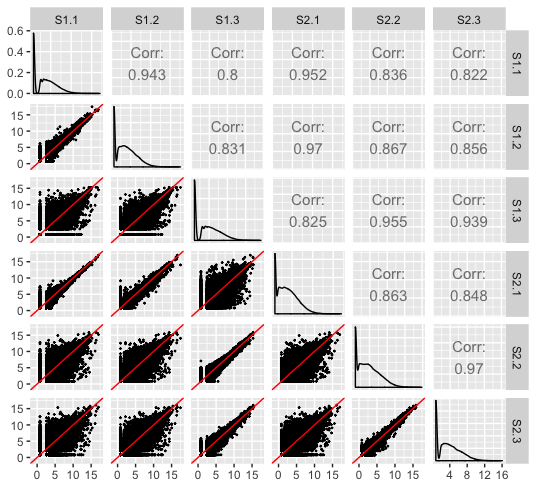
\includegraphics[width=\columnwidth]{MakeFigures/sbCNSwitchedSM.jpg}}
\caption{As expected, this scatterplot matrix contains nine scatterplots with thicker distributions (should be treatment pairs) and six scatterplots with thinner distributions (should be replicate pairs). However, two samples appear to cause a subset of scatterplots to unexpectedly show thicker distributions between replicate pairs and thinner distributions between treatment pairs. If we switch the labels of these two suspicious samples (S1.3 and S2.1), the scatterplot matrix then displays the anticipated structure we saw in Figure~\ref{sbCNSM}. At this point, we have evidence that these two samples may have been mislabeled, and we may wish to confirm this suspicion and correct it before continuing with the analysis.
\label{sbCNSwitchedSM}}
\end{figure}

\begin{figure}[!tpb]
\centerline{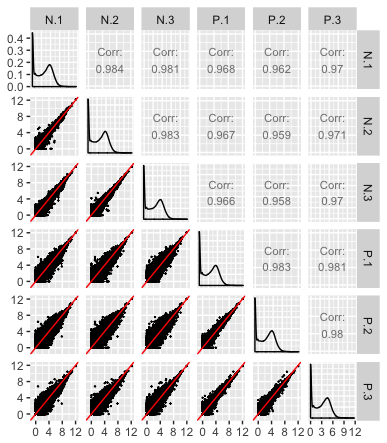
\includegraphics[width=\columnwidth]{MakeFigures/sbIRStreak.jpg}}
\caption{Scatterplot matrix of RNA-seq read counts from soybean leaves after exposure to iron-sufficient (treatment group P) and iron-deficient (treatment group N) soil conditions~\citep{Lauter16}. We observe the expected structure of treatment pairs showing larger variability around the \textit{x=y} line than replicate pairs. However, we notice a pronounced streak structure in the bottom-right scatterplot that compares two replicate samples from the iron-sufficient group. The genes in the streak structure have large read counts that deviate in a parallel fashion from the \textit{x=y} line. Through contacting the authors of this dataset, we discovered that a leaf on one of these samples was inadvertently torn and then documented as such during the experiment. Hence, the genes within this streak structure might represent those that responded to this leaf-tearing event, an observation discovered through the scatterplot matrix that could solidify into a post-hoc hypothesis.
\label{structure}}
\end{figure}

\subsection{Assessing differential expression calls in scatterplot matrices}

The scatterplot matrix can also be used to quickly examine the DEGs returned from a given model. Figure~\ref{sbIRDEG} shows the DEGs from the soybean cotyledon dataset superimposed as orange points onto the scatterplot matrix. We expect for DEGs to fall along the \textit{x=y} line for scatterplots between replicates and deviate from the \textit{x=y} line for scatterplots between treatment groups, as is confirmed in Figure~\ref{sbIRDEG}. As a side note, we can also link these DEGs as parallel coordinate lines on a side-by-side boxplot like in Figure~\ref{sbIRDEG} to confirm the expected pattern of differential expression from a second viewpoint. If we do not observe what should be expected of DEGs, then the DEG calls from the model may need to be scrutinized further.

As an additional example, we overlaid the significant genes from the four clusters of the iron-metabolism soybean dataset (originally shown in Figure~\ref{sbIRClustersSig}) onto the scatterplot matrix. The results are shown and briefly discussed in Supplementary Figures 2-5. 

\section{Litre plots}

We demonstrated how to view differentially expressed genes onto the Cartesian coordinates of the scatterplot matrix in Figure~\ref{sbIRDEG}. Unfortunately, this figure becomes limited when we investigate treatment groups that contain a large number of replicates because we then have too many small scatterplots for it to remain an effective visualization tool. Moreover, researchers could benefit from additional plotting tools that allow them to quickly verify individual differentially expressed genes returned from a model. As a result, we developed a plot that allows users to visualize \textit{one} differentially expressed gene of interest onto the Cartesian coordinates of \textit{one} scatterplot matrix.

The ``replicate line plot" was developed by a group of researchers who demonstrated it could detect model scaling problems in microarray data \citep{Cook}. Unfortunately, this plot is only applicable on datasets where treatment groups contain exactly two replicates. The plot we now introduce is an extension of the ``replicate line plot" that can be applied to datasets with two or more replicates. We call this new plot a repLIcate TREatment (``litre") plot.

In the litre plot, each gene is plotted once for each possible combination of replicates between treatment groups. For example, there are nine ways to pair a replicate from one treatment group with a replicate from the other treatment group in the soybean iron-metabolism dataset (N.1 and P.1, N.1 and P.2, N.1 and P.3, N.2 and P.1, N.2. and P.2, N.2 and P.3, N.3 and P.1, N.3 and P.2, and N.3 and P.3). Hence, a given gene from this dataset is plotted as nine points in the litre plot. With 56,044 genes in this dataset, we would need to plot 504,396 points. This would reduce the speed of interactive functionality as well as cause overplotting problems. As a result, we again use hexagon bins to summarize this massive information (Figure~\ref{repDot} shows four example litre plots).

Once the background of hexagons has been drawn to give us a sense of the distribution of all treatment pair combinations for all genes, the user can superimpose the nine points of one gene of interest. We can examine and compare litre plots using the clusters we created in Figure~\ref{sbIRClustersSig}. Subplots A and B of Figure~\ref{repDot} each show a significant gene from Cluster 2 plotted as nine mustard points, subplots C and D each show a significant gene from Cluster 3 plotted as nine pink points, and subplots E and F each show a significant genes from Cluster 4 plotted as nine coral points. Note that, in the examples in Figure~\ref{repDot}, the read counts of treatment pair combinations sometimes overlap, resulting in the appearance of less than nine points being overlaid. Example litre plots from Cluster 1 are shown in Supplementary Figure 7.

\begin{figure}[!tpb]
\centerline{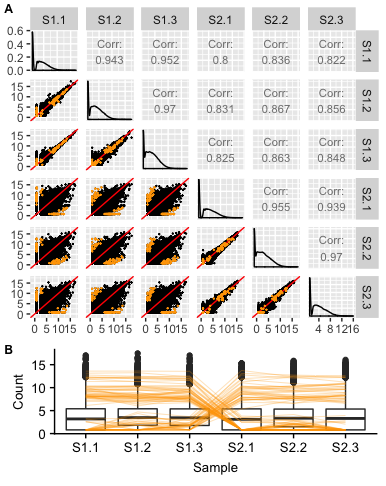
\includegraphics[width=\columnwidth]{MakeFigures/sbIRDEG.jpg}}
\caption{Example of the expected structure of DEG calls (in orange) from an RNA-seq dataset. In the scatterplot matrix (subplot A), DEGs should fall along the \textit{x=y} line for replicates and deviate from it for treatments. In the parallel coordinate plot (subplot B), DEGs should show levelness between replicates and crosses between treatments. These two plotting types can be linked to quickly provide users multiple perspectives of their DEG calls.
\label{sbIRDEG}}
\end{figure}

\begin{figure}[!tpb]
\centerline{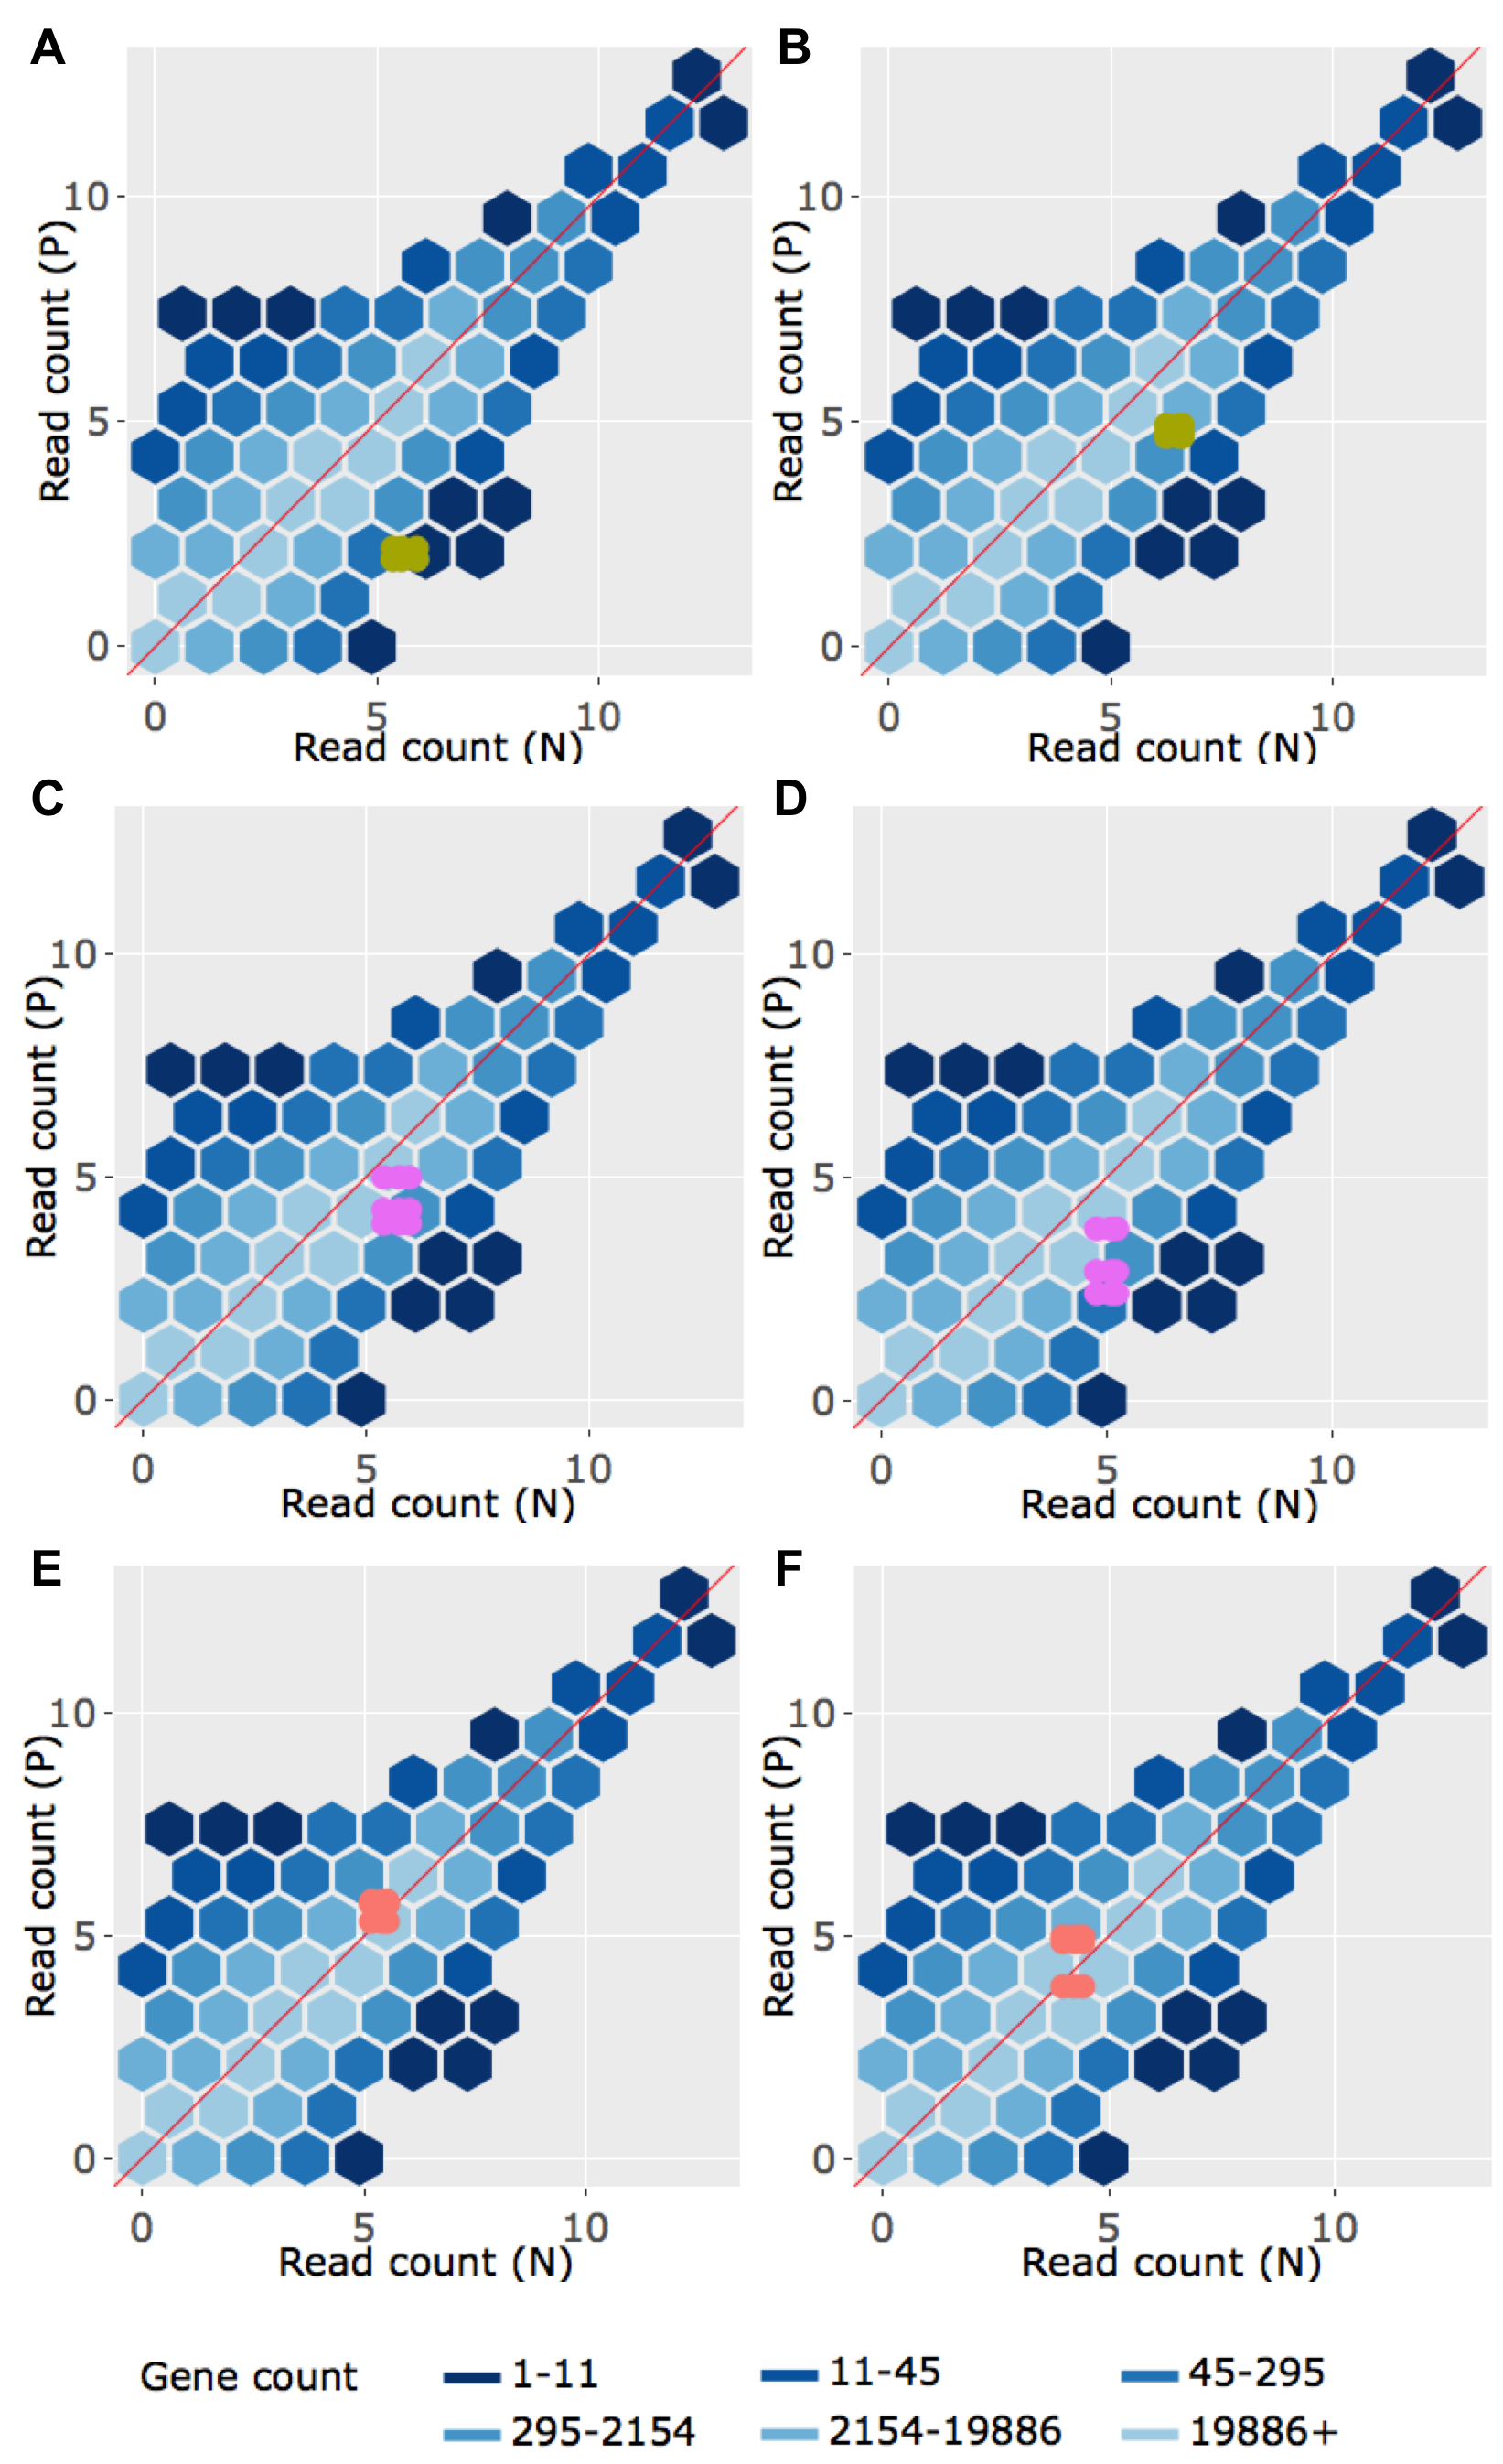
\includegraphics[width=\columnwidth]{MakeFigures/litre6LB.png}}
\caption{Litre plots for representative genes from clusters created in Figure~\ref{sbIRClustersSig}. Subplots A and B each show a gene from Cluster 2 overlaid as nine mustard points. Subplots C and D each show a gene from Cluster 3 overlaid as nine pink points. Subplots E and F each show a gene from Cluster 4 overlaid as nine coral points. Litre plots allow us to quickly flip through genes and search for (possibly odd) patterns that may not be detected numerically.
\label{repDot}}
\end{figure}

For the case of Figures~\ref{repDot} A and B, the nine overlaid points are superimposed in a manner we would expect from a differently expressed gene: They are located far from the \textit{x=y} line (difference between treatments) and are close to each other (similarity between replicates). In fact, the replicates in subplot B are so precise that the overlaid points almost entirely overlap each other. In contrast, Figures~\ref{repDot} C and D do not seem to show as much replicate consistency. Now, there seems to be a pattern in which one replicate from the P group is larger than (and visually distanced from) the other two replicates. In other words, litre plots are able to capture the pattern differences in the significant genes from Cluster 2 and 3 that we saw back in Figure~\ref{sbIRClustersSig}.

Moreover, in the case of Figures~\ref{repDot} E and F, the nine overlaid points are not clearly superimposed in the distinct pattern we expect of significant genes. While subplot E shows a gene that has consistent replications, the difference between the treatment groups is so small that the overlaid points cluster around the \textit{x=y} line. Additionally, the gene displayed in subplot F shows inconsistent replications and consistent treatment groups, as the spread-out overlaid points center on the \textit{x=y} line. Despite these genes being deemed significant by the model, the litre plots call into question whether the genes from this cluster show an expected profile of differential expression. This is similar to the messy-looking parallel coordinate plots we saw from these genes in Cluster 4 back in Figure~\ref{sbIRClustersSig} and the messy-looking superimposition we saw from these genes in Cluster 4 onto the scatterplot matrix in Supplementary Figure 5. As a result, litre plots can detect odd and questionable patterns in individual ``significant genes" that cannot be detected numerically through models. If this happens, the user may wish to further investigate these DEG calls.

The interactive litre plot for the Cluster 2 significant genes (Figure~\ref{repDot} A and B) is available at https://rnaseqvisualization.shinyapps.io/litreCluster2, the interactive litre plot for the Cluster 3 significant genes (Figure~\ref{repDot} C and D) is available at https://rnaseqvisualization.shinyapps.io/litreCluster3, and the interactive litre plot for the Cluster 4 significant genes (Figure~\ref{repDot} E and F) is available at https://rnaseqvisualization.shinyapps.io/litreCluster4. As can be verified in the interactive version of the litre plot, users are provided several input fields that tailor the plot functionality. For instance, the user may wish to quickly scroll through significant genes one by one in the order of lowest to highest FDR values. Please read the ``About" tab in the interactive links for more information.

\section{Closing case study}

We briefly discuss an additional example that merges many of the topics addressed in this paper. The publicly available data for this example contain technical replicates of liver and kidney RNA samples \citep{Marioni}. We first calculate DEG calls for this data using the popular normalization method of library size scaling, where the number of total reads in each sample are normalized to a common value across all samples. This process leads to 9,018 DEGs, with most of them ($\sim$78\%) showing higher expression in the kidney group.

Although we could finish our analysis at this point and draw conclusions based on this list of DEGs that came from the model, it would be wise to also view this dataset visually. Viewing this data as a scatterplot matrix confirms the expected pattern with treatment scatterplots showing larger variation than technical replicate scatterplots. However, it also uncovers a hidden pattern in the treatment plots: There is a pronounced streak of genes with higher expressions in the liver group (Figure~\ref{lkSM}). We should also view the DEGs from the model using parallel coordinate plots: Upon doing so, we notice that while the 1,968 liver-specific DEGs follow the expected pattern of significant calls, a substantial fraction of the 7,050 kidney-specific DEGs appear comparatively noisy (Figure~\ref{lkClusters}A).

\begin{figure}[!tpb]
\centerline{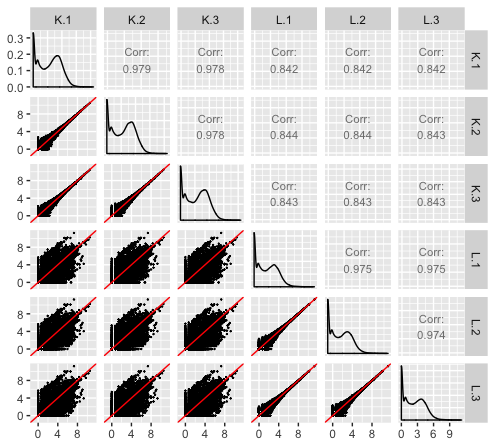
\includegraphics[width=1\columnwidth]{MakeFigures/lkSM.jpg}}
\caption{Scatterplot matrix of liver and kidney technical replicates. The technical replicate scatterplots look precise as is expected, with little variability around the \textit{x=y} line. The treatment group scatterplots have much more variability around the \textit{x=y} line, as we would expect. However, each treatment group scatterplot contains a pronounced streak of highly-expressed liver-specific genes, which deviates from the expected distribution. Some researchers have suggested that differences in the distribution of reads between groups may require particularly stringent normalization.
\label{lkSM}}
\end{figure}

\begin{figure}[!tpb]
\centerline{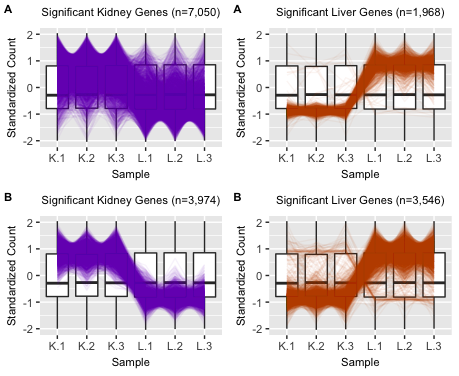
\includegraphics[width=1\columnwidth]{MakeFigures/lkClusters.jpg}}
\caption{Subplot A shows parallel coordinate plots of the DEGs from liver and kidney technical replicates after standard library scale normalization. The division of DEGs between the two groups was rather disparate, with ~78\% of the DEGs being kidney-specific and only ~22\% of the DEGs being liver-specific. Also of note, while the parallel coordinate patterns of the liver-specific DEGs appear as expected, the patterns of the kidney-specific DEGs seem to show comparatively larger variability between the replicates. Subplot B shows parallel coordinate plots of the DEGs from liver and kidney technical replicates after TMM normalization. The division of DEGs between the two groups is more balanced than in Subplot A, with ~53\% of the DEGs being kidney-specific and ~47\% of the DEGs being liver-specific. Additionally, the parallel coordinate patterns of both the liver-specific and kidney-specific DEGs appear as expected and more consistent with each other.
\label{lkClusters}}
\end{figure} 

Taking both of these observations into account, we may need to reconsider our normalization technique. Some authors have argued that the popular library scaling method is not adequate in all cases, especially when the underlying distribution of reads between samples is inconsistent. In the current data, the observed streak of outlier genes that are highly expressed in the liver samples reduces the sequencing quota available to the remaning genes in these samples, which could create an articial inflation of the kidney-specific DEG calls. These authors have recommended TMM normalization for such cases (including for this particular dataset) as this technique generates sample scaling factors that consider sample distributions \citep{RobinsonOshlack}.

In light of all this, we return to square one and now apply TMM normalization to this data. This process leads to 7,520 DEGs that have a more level distribution between the kidney ($\sim$53\%) and liver ($\sim$47\%) groups. The scatterplot matrix did not appear differently from what we saw in Figure~\ref{lkSM} as both of these normalization methods are scaling procedures. However, we should visualize the new DEG calls. Plotting these DEGs as parallel coordinate lines paints a much cleaner picture from what we saw earlier, with most genes following the expected pattern of significance (Figure~\ref{lkClusters}B). Of the 7,050 kidney-specific DEGs we saw previously with library scaling normalization, only a cleaner-looking subset (n=3,974) of them remained as such using TMM normalization.

A deeper investigation of the effects of normalization on this data are shown in the supplementary material. These visualizations collectively suggest that this datasest indeed requires more than just library scaling for reliable analysis. This case study was meant to underscore the overarching theme of this paper that iteration between models and visualizations is crucial to achieve the most convincing results and conclusions in RNA-seq studies.

\section{Discussion}

In this paper, we strived to convince readers that effective visualization should be a crucial part of RNA-seq analysis. We used real data to demonstrate that scatterplot matrices, parallel coordinate plots, and litre plots can help users check for normalization problems, catch common errors in the analysis pipeline, and confirm that the variation between replicates and treatments is as expected. We also showed that these graphical tools allow researchers to quickly explore lists of DEGs that come out of models and ensure which ones make sense from an additional and arguably more intuitive vantage point. Moreover, we demonstrated that our simple plotting tools allow researchers to discover genes of interest through visual geometric patterns that would otherwise remain undiscovered with models.

In general, scientists might uncover surprising patterns lurking in their data with plots in ways that cannot be achieved with any formulas or models. Researchers from all statistical backgrounds can use graphical tools to better understand (if not demystify) how the application of various normalization techniques and/or models affect their results. All in all, scientists can gain more confidence in the data analysis pipelines they choose and in the results they draw at the mere cost of briefly creating and exploring graphical outputs during their analyses.

Modern data analysis is most reliable when models and visuals are used congruently. Unfortunately, the current culture around RNA-seq analysis de-emphasizes the importance of graphical tools, which, as we have shown, calls into question the soundness of results that come from RNA-seq studies. Solving this problem is simple and does not require scientists to drastically change their approach to RNA-seq analysis. Instead, scientists simply need to incorporate effective plotting tools during their usual analysis pipelines. We plan to serve a role in this solution by publishing a new \textsf{R} software package that includes the useful plotting techniques we introduced in this paper. To encourage scientists to use this resource, we aim to include a straight-forward vignette that demonstrates how to painlessly apply these graphical tools to RNA-seq data. It is our hope that such work will serve a small part in upgrading the RNA-seq analysis world into one that more wholistically extracts meaningful biological information using both models and visuals.

\section*{Acknowledgements}

R \citep{R} was used to conduct analyses in this paper, and particularly packages ggplot2 \citep{ggplot2}, Shiny \citep{shiny}, plotly \citep{plotly}, and htmlwidgets were used to build the graphics. 

\section*{Funding}

Research of Graham and Moran Lauter was financed by the United States Department of Agriculture, Agricultural Research Service (USDA-ARS) CRIS Project 5030-21220-005-00D and the Iowa Soybean Association.








%%%%%%%%%%%%%%%%%%%%%%%%%%%%%%%%%%%%%% CHAPTER %%%%%%%%%%%%%%%%%%%%%%%%%%%%%%%%%%%%%% 
%%%%%%%%%%%%%%%%%%%%%%%%%%%%%%%%%%%%%%%%%%%%%%%%%%%%%%%%%%%%%%%%%%%%%%%%%%%%%%%%%%%%%

\chapter{Visualization methods for significance testing of RNA-sequencing data}
\label{sec:sigtest}

\section{Future avenues}

We have several avenues we could pursue to expand upon this work:

\begin{enumerate}
\item \textbf{Strengthen normalization}: The MDS plot, scatterplot matrices, and parallel coordinate plots from clustering analysis did not appear as clean in the paper wasp data as they did for soybean data. One method we can approach is a more robust normalization process as outlined in the RUVseq package (\citealt{ruvseq}). Within this approach, there are three possible directions in which a handful of "negative control transcripts" must be used.

\begin{enumerate}
\item \textbf{Housekeeping transcripts}: In this approach, we would use a small number of robust transcripts with known quantities that do not change much from one treatment to another. For the \textit{Polistes fuscatus} transcriptome, there are a small number of known transcripts for this purpose (such as actin, rp49, and S8), although their usefulness is dubious as their quantity can vary considerably across different experimental conditions.
\item \textbf{Internal control transcripts}: In this approach, we obtain an "in-silico empirical" set of negative control transcripts by examining the properties of the transcripts within the data itself. This approach is ideal if we cannot obtain a set of negative control transcripts elsewhere.
\item \textbf{Spike-in controls}: In this approach, a known concentration of RNA transcripts are applied. As such, they can be advantageous to endogenous controls. However, we have yet to determine if the RNA-sequencing for this data had employed spike-in controls. 
\end{enumerate}

\item \textbf{Map to genome}: We have so far examined the transcript read counts after the reads were mapped to the transcriptome from the same species (\citealt{pw19}). We could also consider examining the genome read counts by mapping the reads to the genome of a similar species.

\item \textbf{Permutation testing}: Although the top differentially expressed transcripts between DU and DR looked promising (in Figure \ref{fig:degPW}), we will also develop permutation testing for this type of visual analysis of differentially expressed transcripts. Namely, we can create permutations where the sample names (DU.1, DU.2, ..., DR.6) are randomly assigned to columns in the data. After that, we can rerun the edgeR process on this falsely-named data, determine the new set of differentially expressed transcripts, and examine this new set visually with the same plots as in Figure \ref{fig:degPW}. At this point, we can create a lineup of the most statistically-significantly differentially expressed transcripts from the real dataset and from two permuted datasets. This would create a "triplet plot", where the location of the actual data plot is randomized amongst the two permuted data plots. If the actual data plot can be distinguished from the permuted data plots, then we have evidence that the differential expression we found was more due to treatment differences than other differences. This type of visualization inference has been successfully explored in previous work (\citealt{extra6}). To accomplish this, we plan on using the \pkg{nullabor} package (\citealt{nullabor}), which has been successfully used for RNA-sequencing visualization inference (\citealt{extra1}).

\item \textbf{Render plotting interactive}: It would be useful to allow for the permutation testing visualization tools to have an interactive element. For example, users could quickly glance through the triplet plots of the top differentially expressed transcripts to discover if there are any transcripts that appear suspicious. Or, they could quickly rerun the permutation testing on a different set of treatment groups of interest.

\end{enumerate}

The paper wasp data did not respond as well as the soybean data did to the visual tools for RNA-sequencing clustering analysis (which we did not explicitly show in this thesis proposal). This may be due to the fact that the soybean replicates were clones, whereas the wasp replicates were not clones. Moreover, the soybean data is more controlled than the wild paper wasps. It could also be due to us using transcript read counts for the paper wasp data, while we used gene read counts for the soybean data. While there is only negligible overlap between transcripts, there is no longer independence as multiple transcripts can map to the same gene.

However, we have preliminary plotting tools for RNA-sequencing significance testing analysis. We could see that the top differentially expressed transcripts did appear as we would expect in Figure \ref{fig:degPW}. We can now expand upon this by creating interactive permutation testing visualizations of these differentially expressed transcripts.

\chapter{Timeline}
\label{sec:timeline}

\section{Completed}

\begin{tabular}{|p{3cm}|p{8cm}|p{3cm}|}
 \hline
 \textbf{Product} & \textbf{Description} & \textbf{Date} \\ 
 \hline
 R package & First release of \pkg{ggenealogy}, which provides visualization tools for genealogical datasets & March 2015 \\
 \hline
 Presentation & Presented \pkg{ggenealogy} at JSM & August 2015 \\
 \hline
 Award & Student paper award at ASA Statistical Computing and Graphics Section & August 2015 \\
 \hline
\end{tabular}

\section{Scheduled deliverables}

\begin{tabular}{|p{3cm}|p{8cm}|p{3cm}|}
 \hline
 \textbf{Product} & \textbf{Description} & \textbf{Date} \\ 
 \hline
 R package & Second release of \pkg{ggenealogy} package, which provides visualization tools for genealogical datasets & May 2016 \\
 \hline
 Paper & Submit \pkg{ggenealogy} paper to JSS & May 2016 \\
 \hline
 R package & First release of package that provides visualization tools for RNA-sequencing datasets & TBD \\
 \hline
 Paper & Submit paper about visualization tools for clustering analysis of RNA-sequencing & TBD \\
 \hline
 Paper & Submit paper about visualization tools for significance testing of RNA-sequencing & TBD \\
 \hline
\end{tabular}

\section{Other work}

\begin{tabular}{|p{3cm}|p{8cm}|p{3cm}|}
 \hline
 \textbf{Product} & \textbf{Description} & \textbf{Date} \\ 
 \hline
 R package & First release of ePort package that generates electronic reports for instructors to evaluate student performance & July 2016 \\
 \hline
\end{tabular}

\bibliography{myThesis}

\end{document}
